\subsection{Faraday-Pockels}
\subsubsection{Inspection without applied field}
\paragraph{Diffraction and Bifringence}
The inspection of the experimental setup revealed certain aspects
which we might need to include in our interpretation of the results
later. First we noticed minor diffraction phenomena already between
the exit of the Laser's Gaussian Beam and the beginning of the
Pockelcell, as well as bifringence phenomena which caused difficulties
in focusing the laser.  
\paragraph{Low frequency oscillations} Within the lasersignal 
we observed frequencies about $20 Hz$ with a intensity of $10mV/$diff.
We did not expect these frequencies at first; we will look into it
in the later progress of the experiment.
\subsubsection{Calibration of the Analysator with sawtooth wave}
We did now certain measurements for analyzing the behaviour of a 
certain degree of the analysator.
\newcommand{\picwidth}{0.49\textwidth}

\begin{figure}
    \begin{subfigure}[b]{\picwidth}
        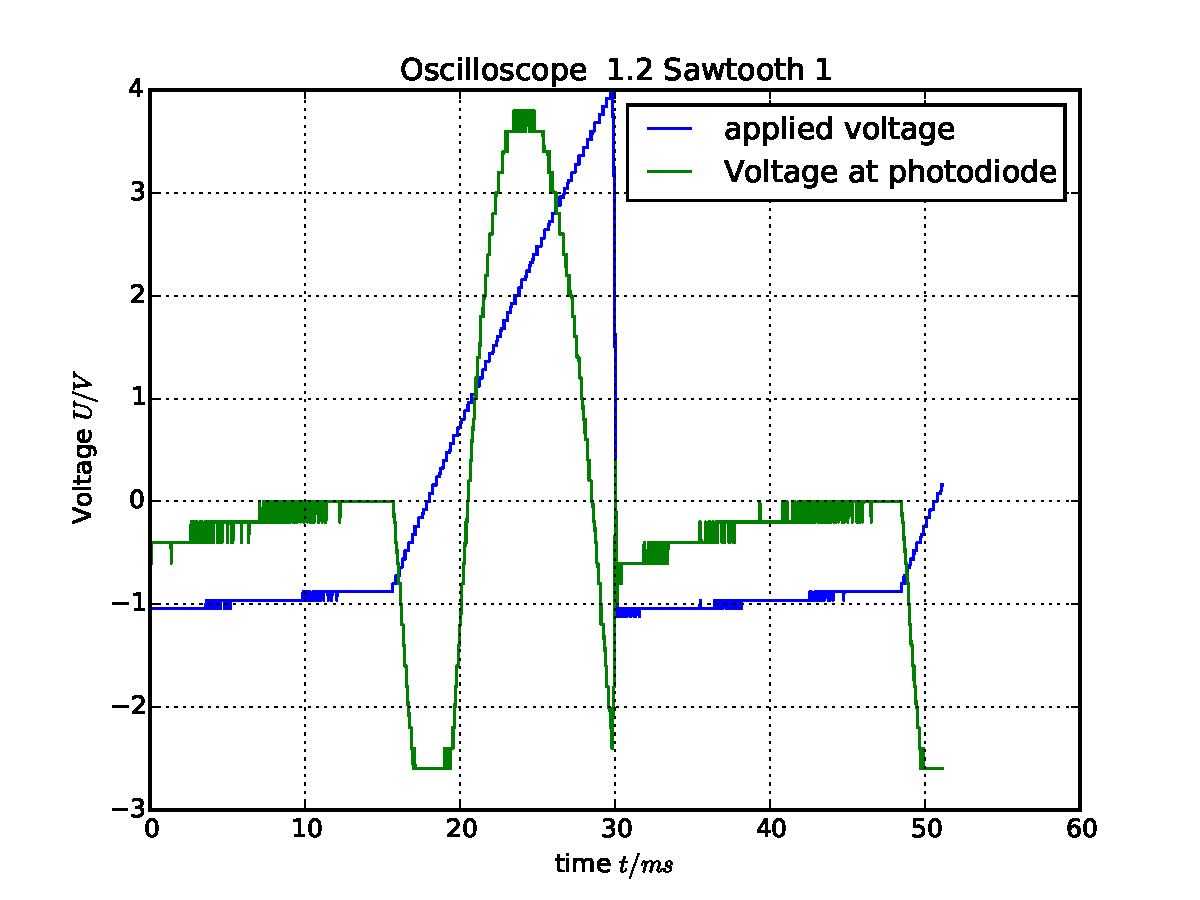
\includegraphics[width=\textwidth]{analysis/figures/12sawtooth1}
        \caption{}
    \end{subfigure}\qquad
    \begin{subfigure}[b]{\picwidth}
        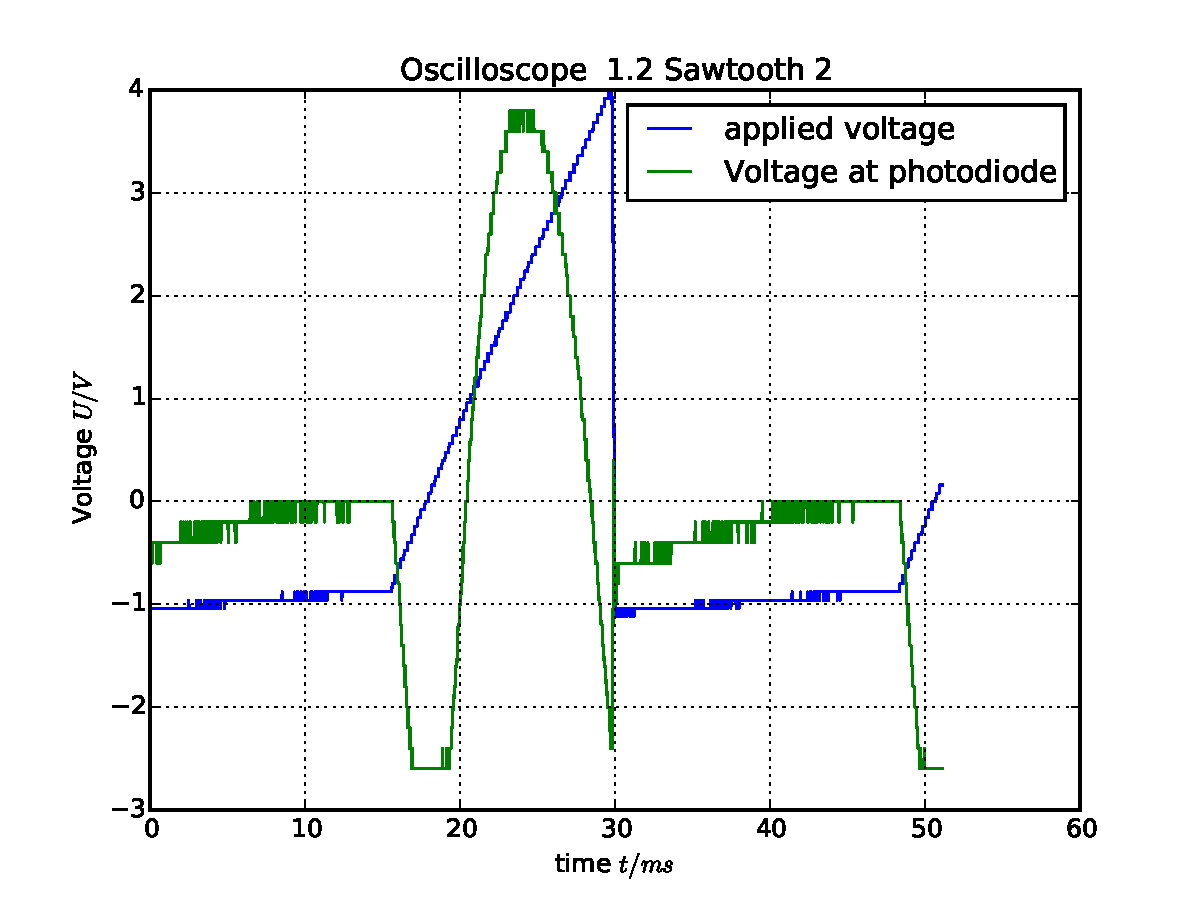
\includegraphics[width=\textwidth]{analysis/figures/12sawtooth2}
        \caption{}
    \end{subfigure}
    \begin{subfigure}[b]{\picwidth}
        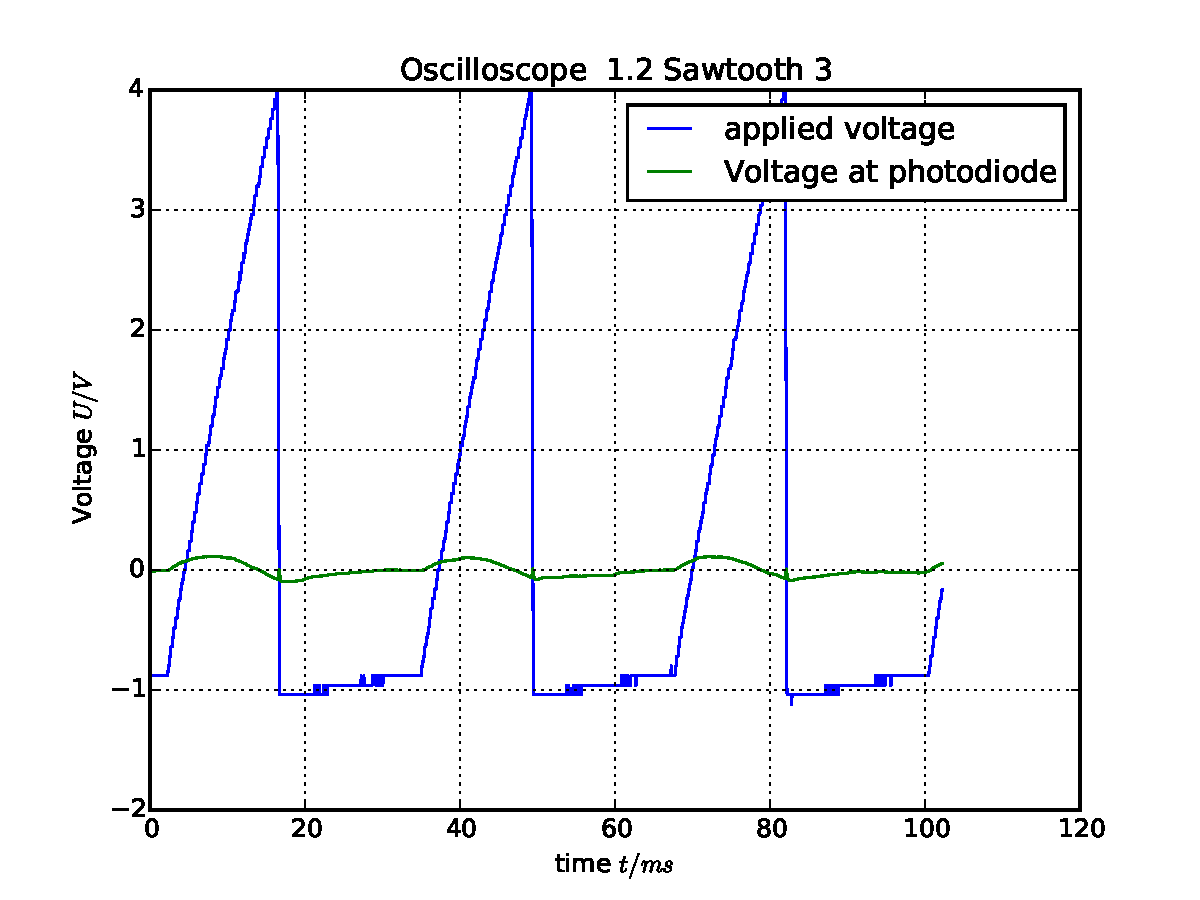
\includegraphics[width=\textwidth]{analysis/figures/12sawtooth3}
        \caption{}
    \end{subfigure}
    \begin{subfigure}[b]{\picwidth}
        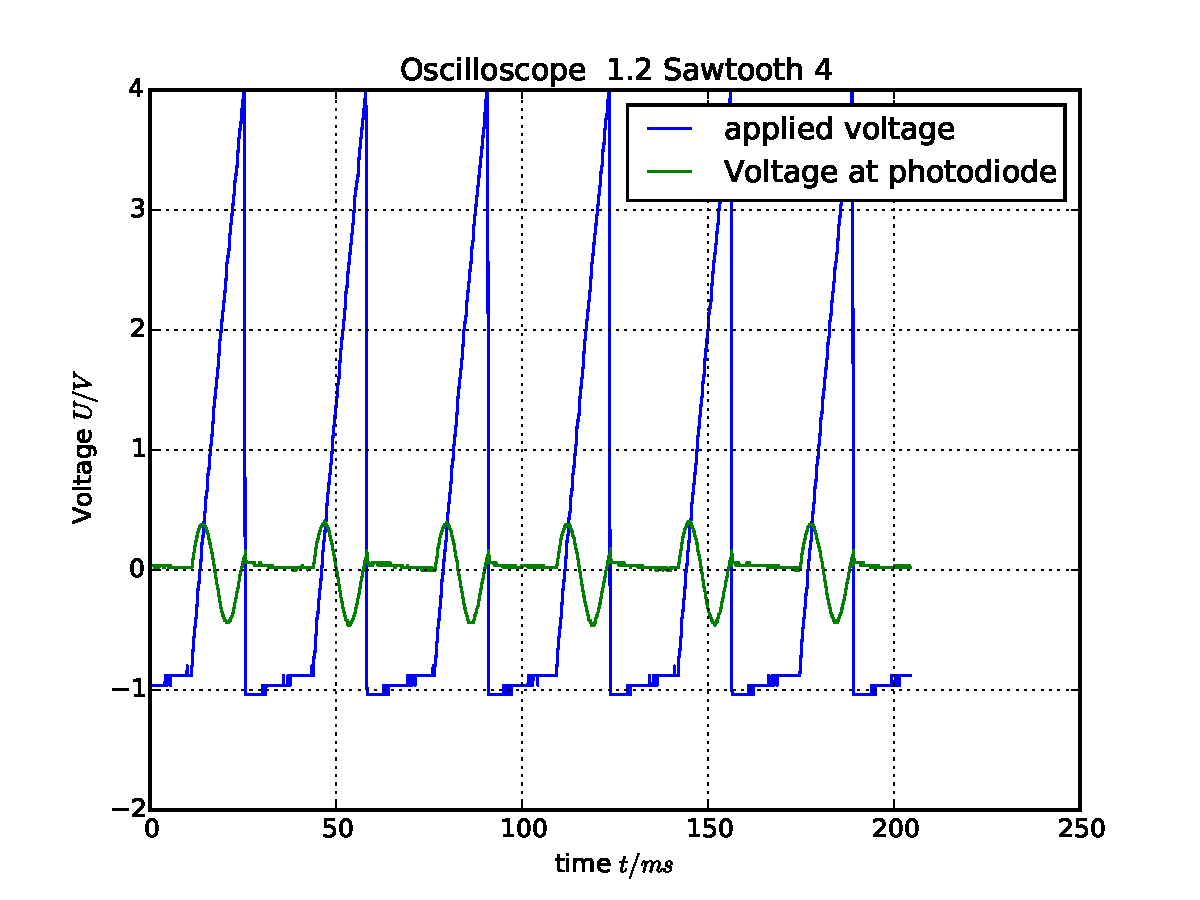
\includegraphics[width=\textwidth]{analysis/figures/12sawtooth4}
        \caption{}
    \end{subfigure}
    \caption{These were the first measurements with the 
        oscillscope in order to calibrate the Analysator.
        The next measurements will show the result of the 
        final calibration. You can find the same configuration
        with different zoom from (b) to (d).}
    \label{fig:saw1}
\end{figure}
\flushleft
\begin{figure}
    \begin{subfigure}[b]{\picwidth}
        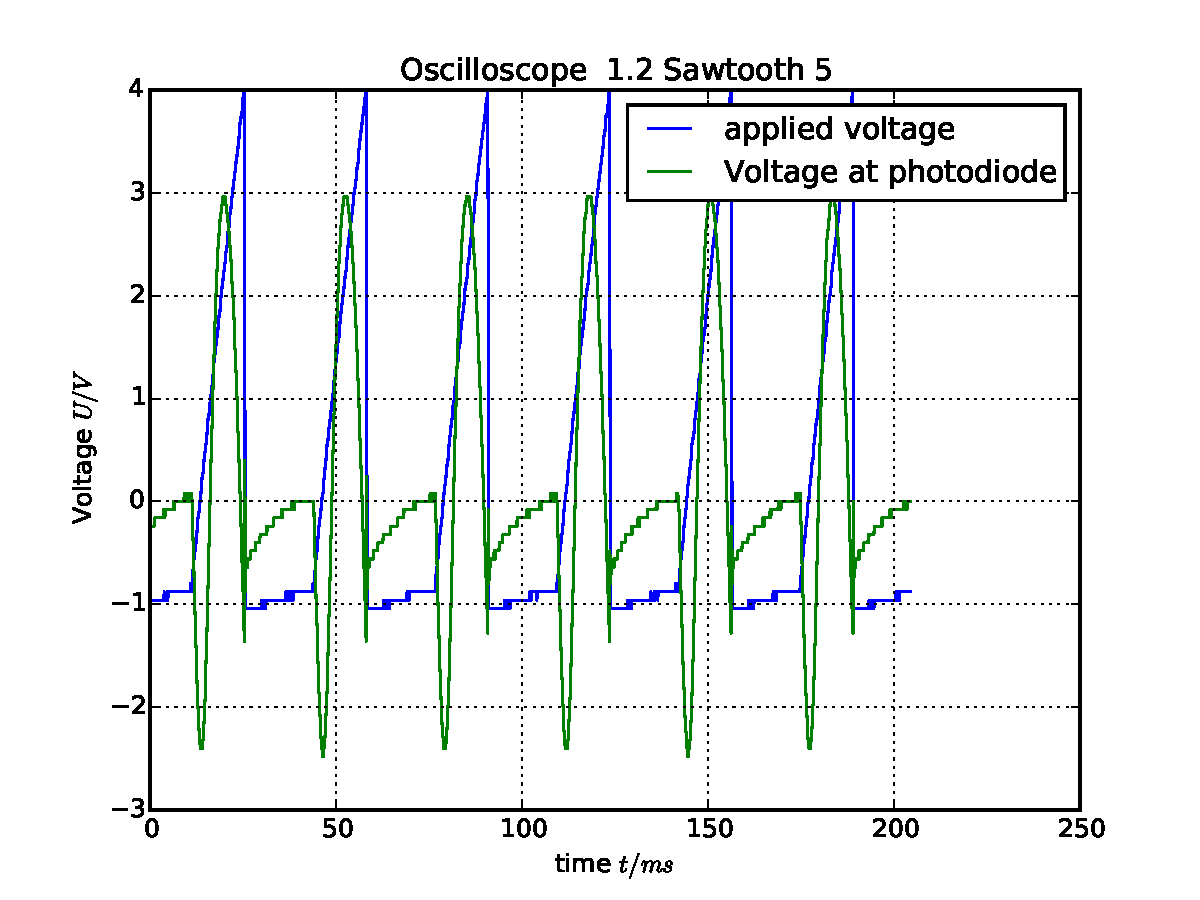
\includegraphics[width=\textwidth]{analysis/figures/12sawtooth5}
        \caption{}
    \end{subfigure}\qquad
    \begin{subfigure}[b]{\picwidth}
        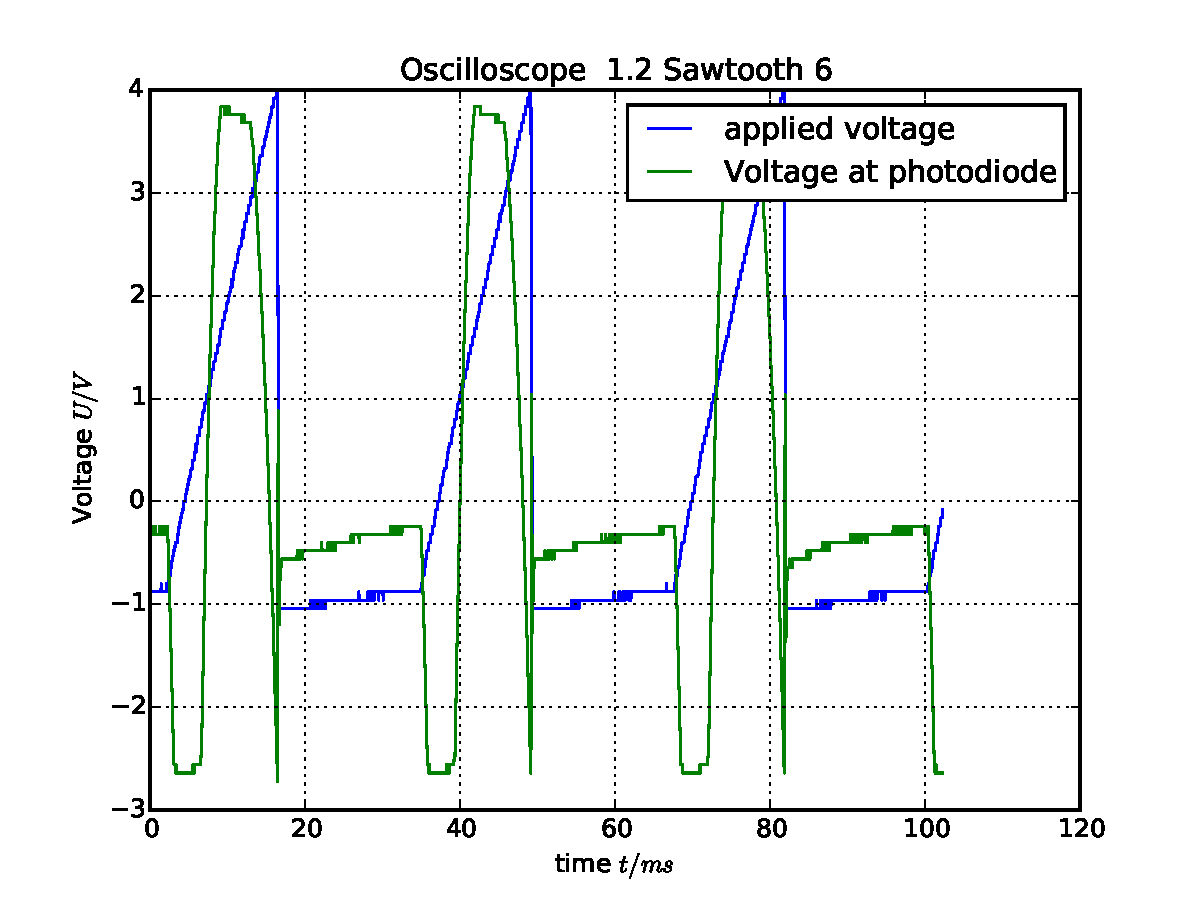
\includegraphics[width=\textwidth]{analysis/figures/12sawtooth6}
        \caption{}
    \end{subfigure}
    \begin{subfigure}[b]{\picwidth}
        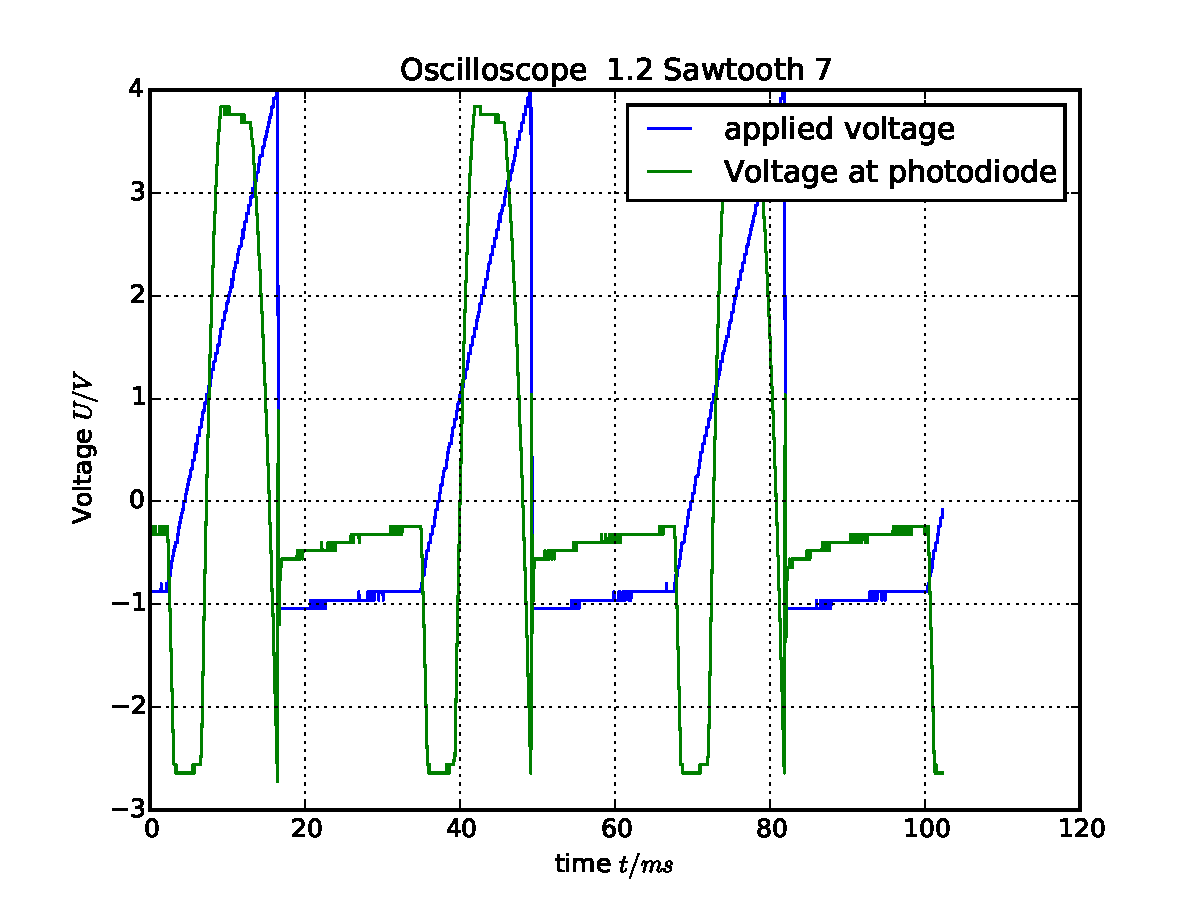
\includegraphics[width=\textwidth]{analysis/figures/12sawtooth7}
        \caption{}
    \end{subfigure}
    \begin{subfigure}[b]{\picwidth}
        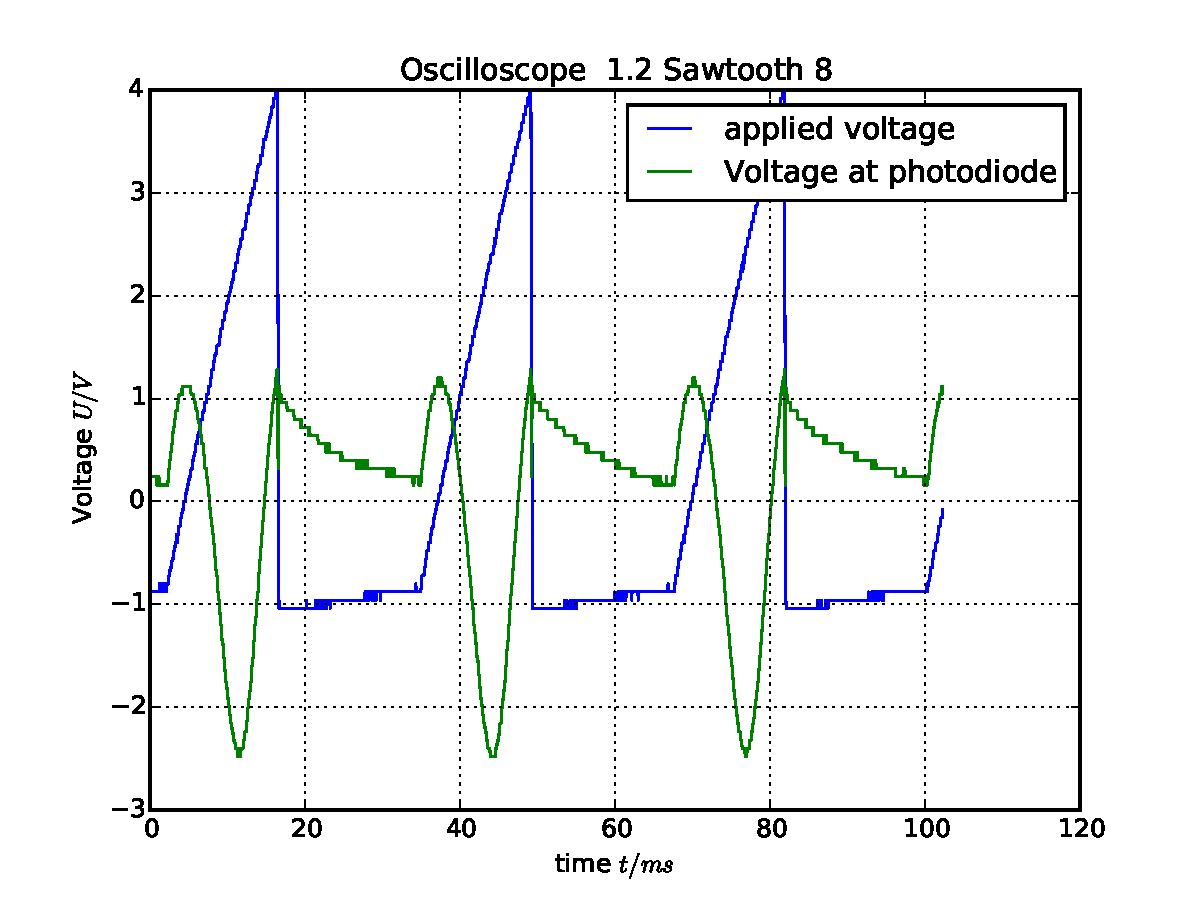
\includegraphics[width=\textwidth]{analysis/figures/12sawtooth8}
        \caption{}
    \end{subfigure}
    \begin{subfigure}[b]{\picwidth}
        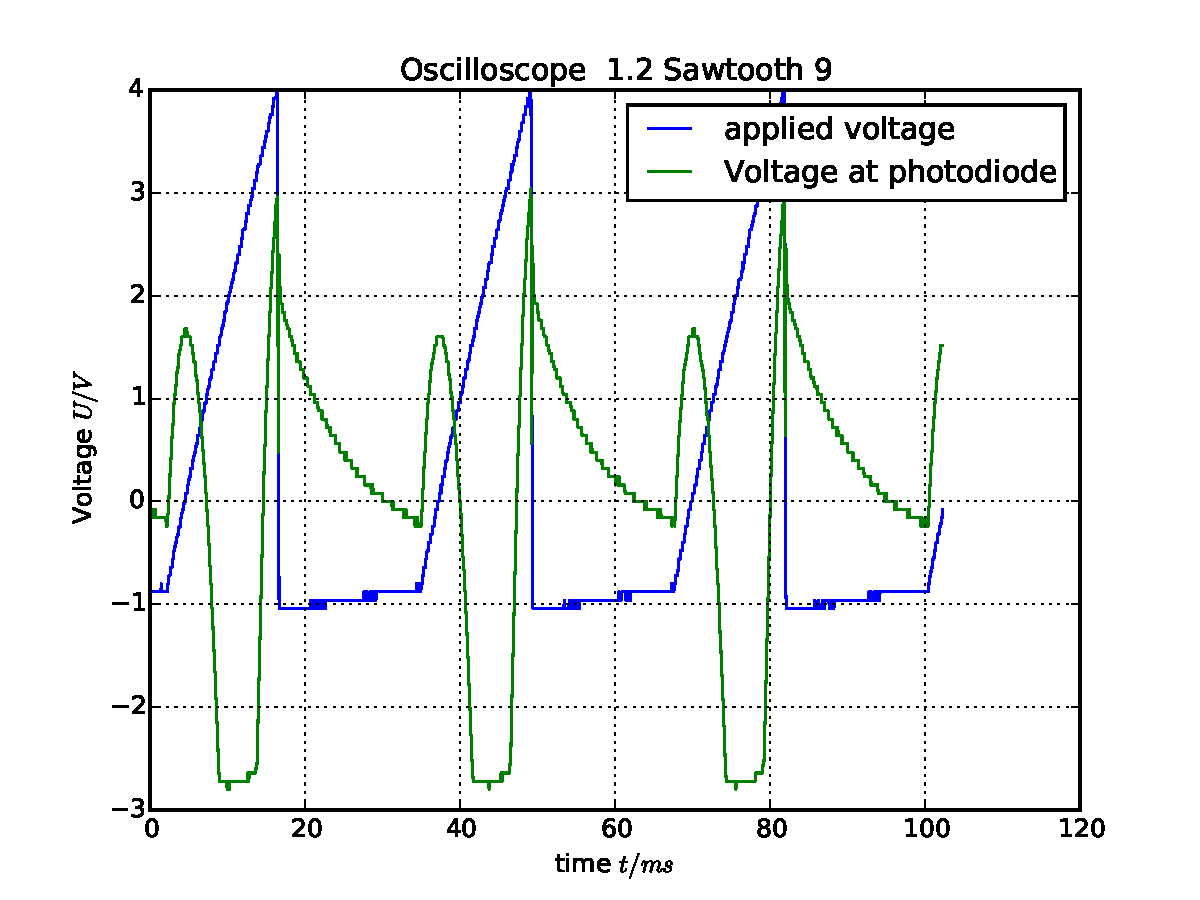
\includegraphics[width=\textwidth]{analysis/figures/12sawtooth9}
        \caption{}
    \end{subfigure}
    \begin{subfigure}[b]{\picwidth}
        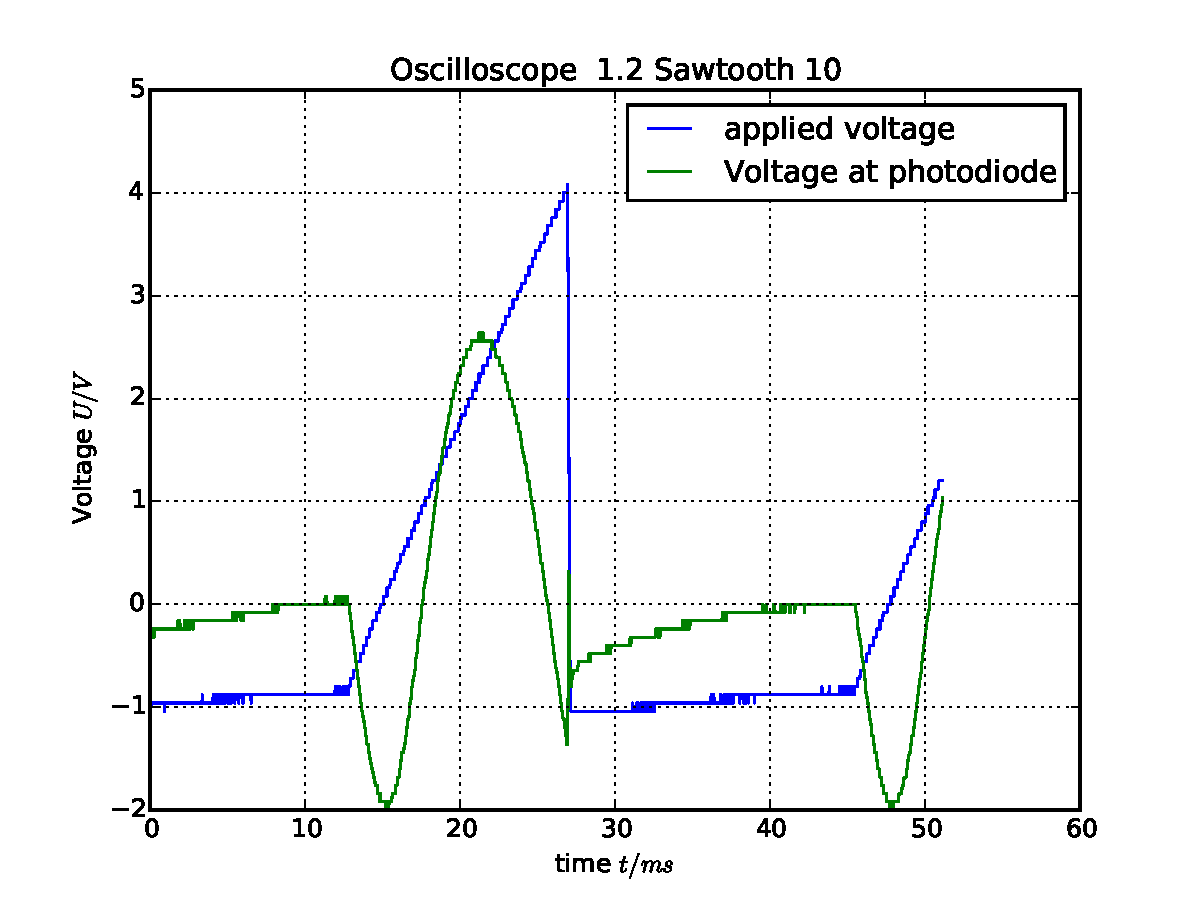
\includegraphics[width=\textwidth]{analysis/figures/12sawtooth10}
        \caption{}
    \end{subfigure}

    \caption{These series of figures show the further 
        attempts to calibrate the analysator. As you can
        notice every figure shows a different degree of the 
        angle and hence the distribution of voltage changes. }
    \label{fig:saw2}
\end{figure}
\flushleft

\begin{figure}
    \begin{subfigure}[b]{\picwidth}
        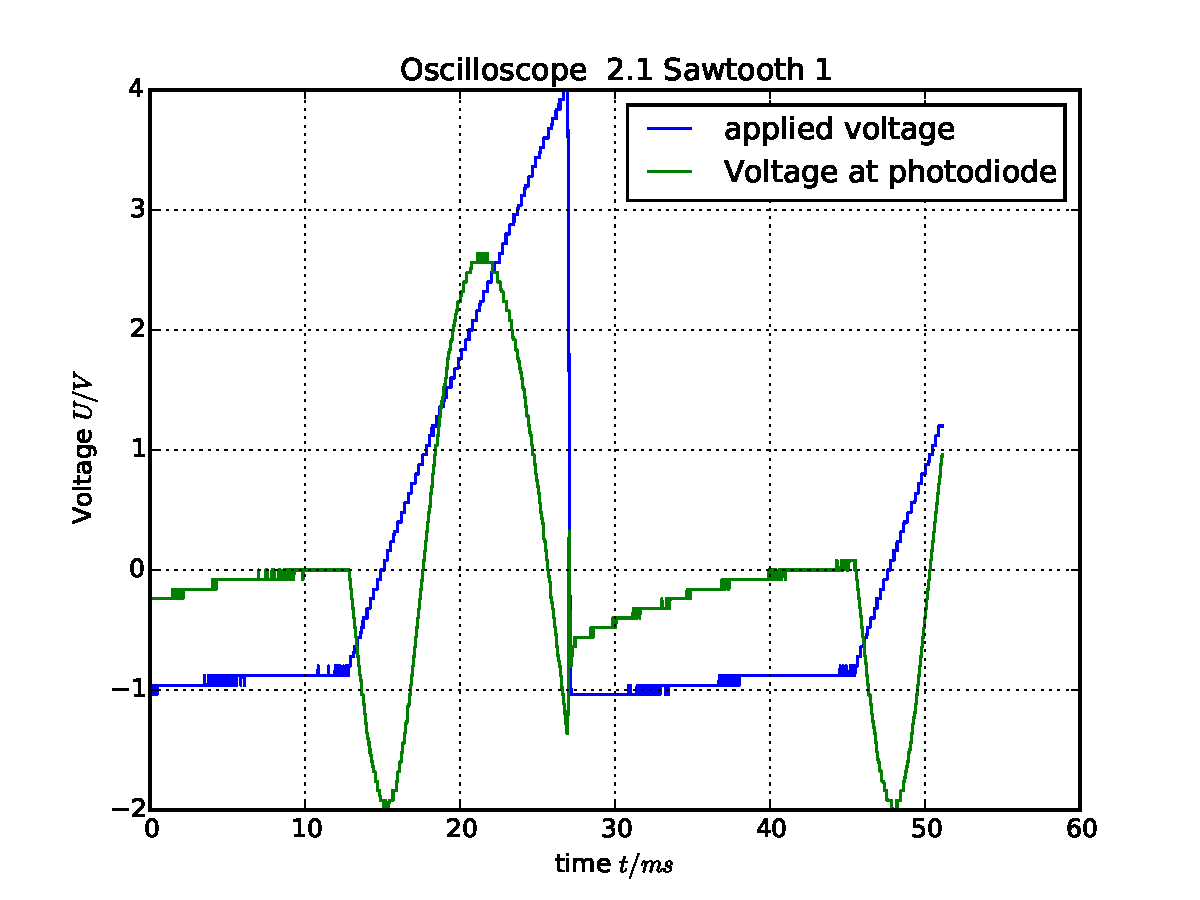
\includegraphics[width=\textwidth]{analysis/figures/21sawtooth1}
        \caption{}
    \end{subfigure}\qquad
    \begin{subfigure}[b]{\picwidth}
        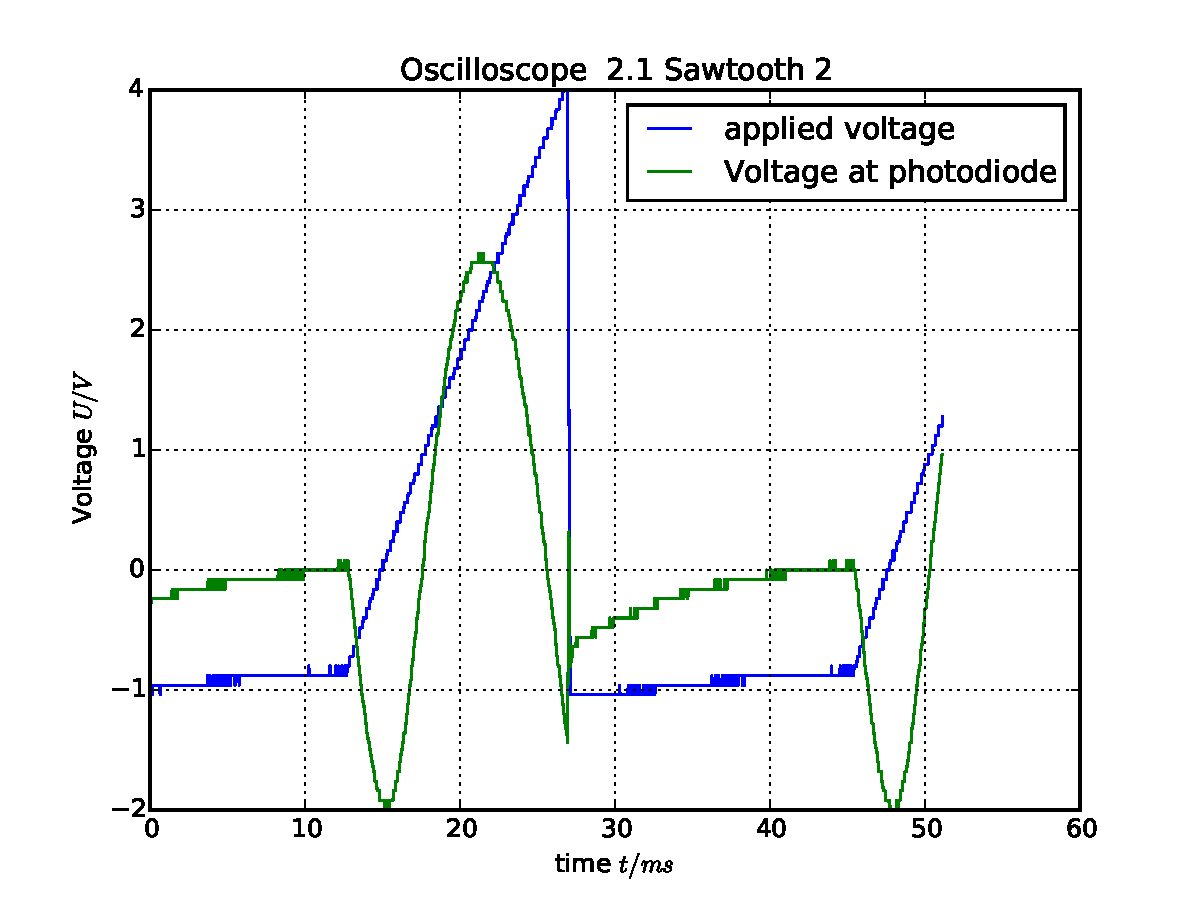
\includegraphics[width=\textwidth]{analysis/figures/21sawtooth2}
        \caption{}
    \end{subfigure}
    \begin{subfigure}[b]{\picwidth}
        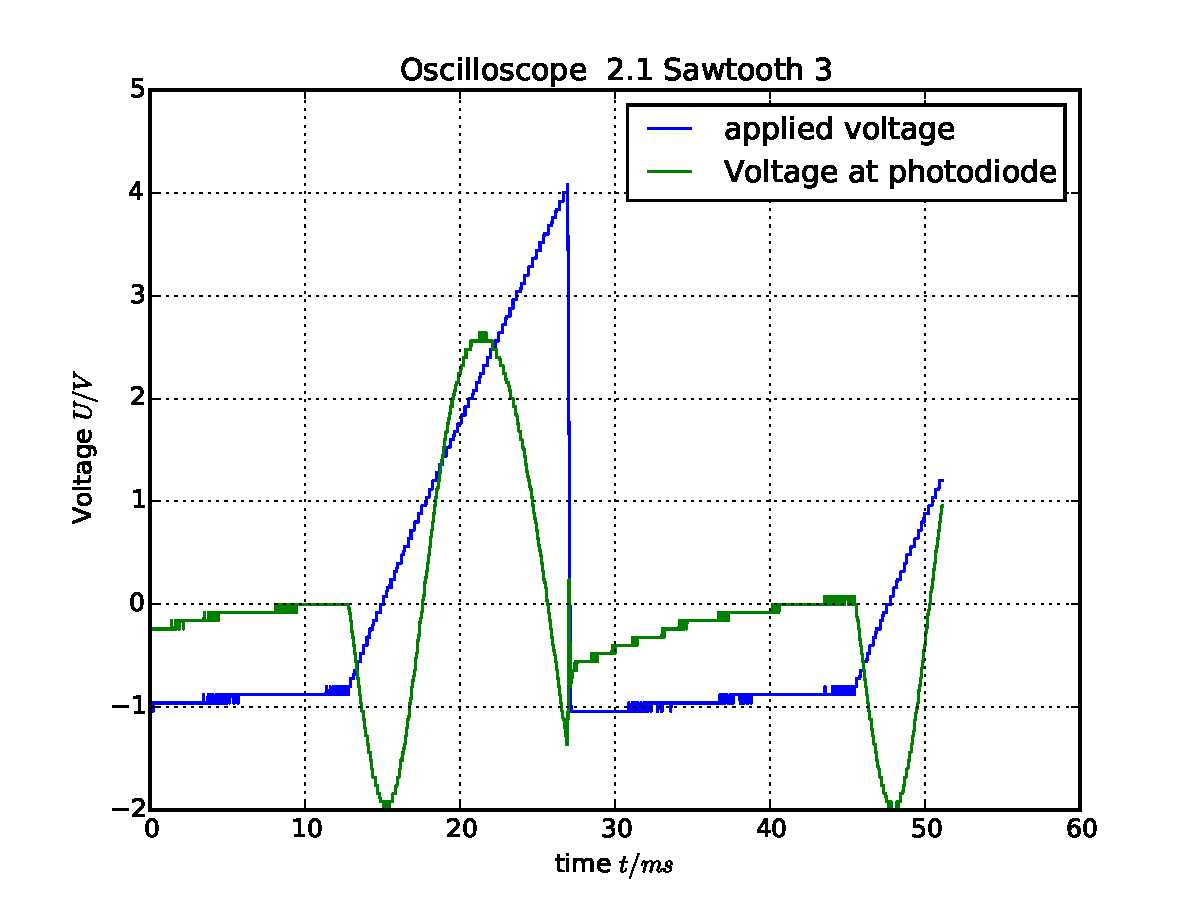
\includegraphics[width=\textwidth]{analysis/figures/21sawtooth3}
        \caption{}
    \end{subfigure}
    \begin{subfigure}[b]{\picwidth}
        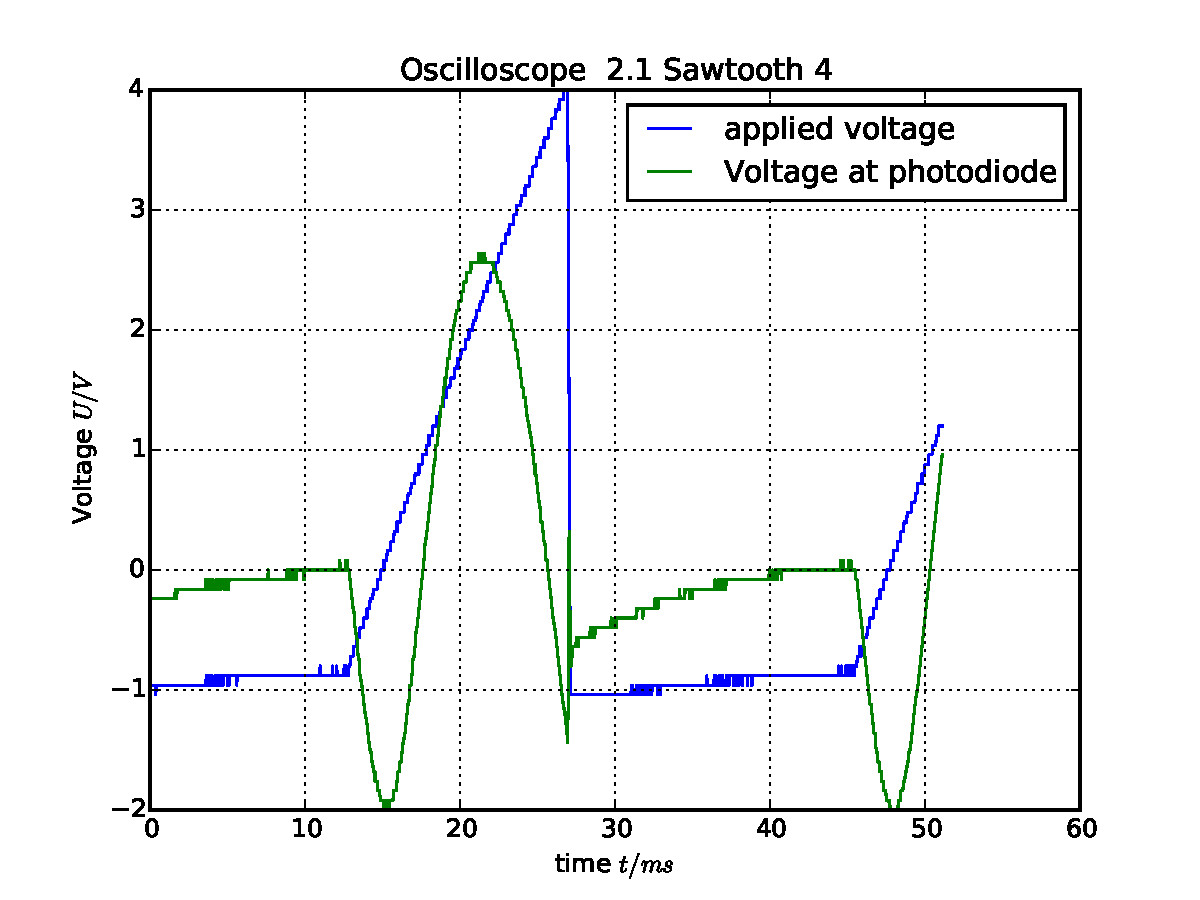
\includegraphics[width=\textwidth]{analysis/figures/21sawtooth4}
        \caption{}
    \end{subfigure}
    \begin{subfigure}[b]{\picwidth}
        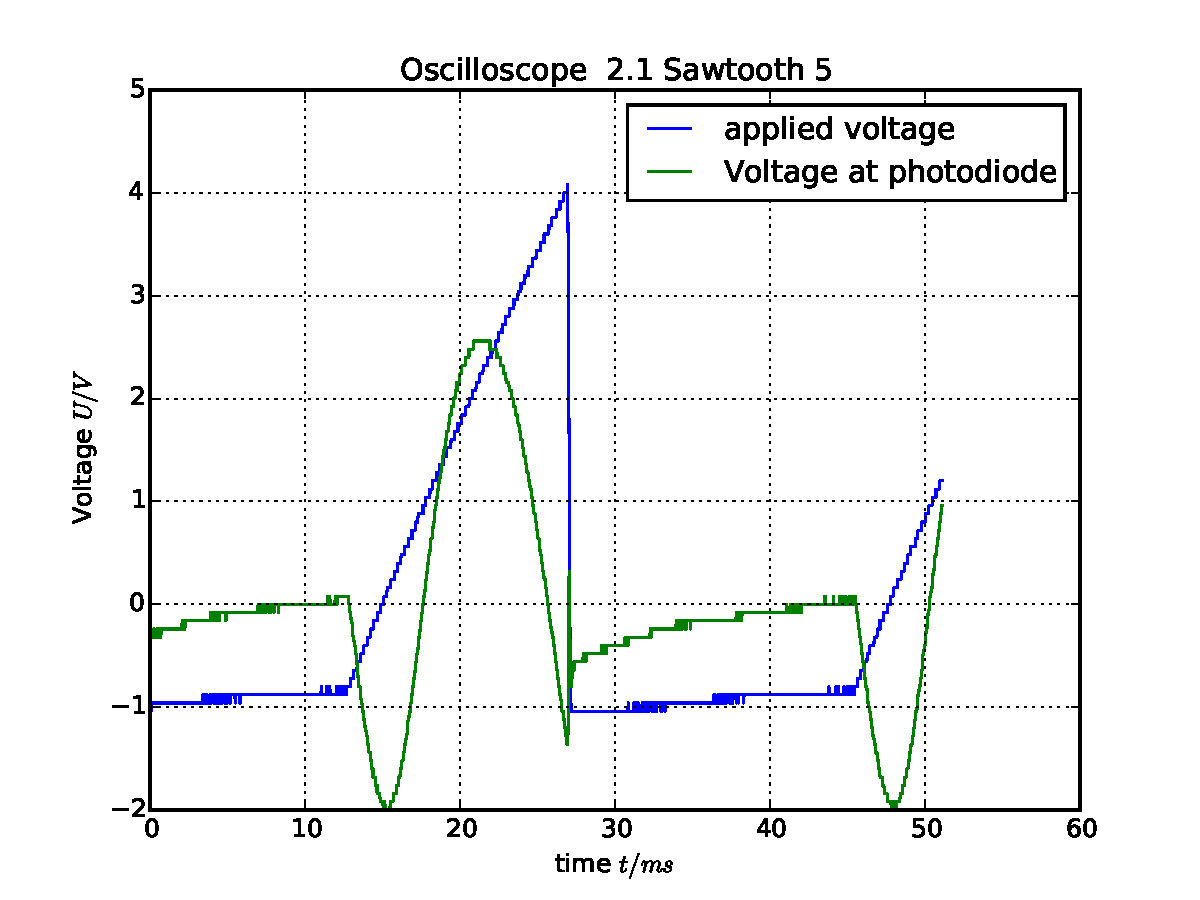
\includegraphics[width=\textwidth]{analysis/figures/21sawtooth5}
        \caption{}
    \end{subfigure}
    \caption{
        This is the final calibration of the analyzer. As you
        can see we did not change the state anymore and all the
        results are in general the same.
        }
    \label{fig:saw3}
\end{figure}
\flushleft
\clearpage
\subsubsection{Sinus-generated Method, without Direct Current}
The Frequency generated was about $f=5.4$ Khz, but it was not stable
but oscillating within $0.1$ Khz. The manipulation of the trigger-
level increased the stability to a acceptable level. 
\begin{figure}
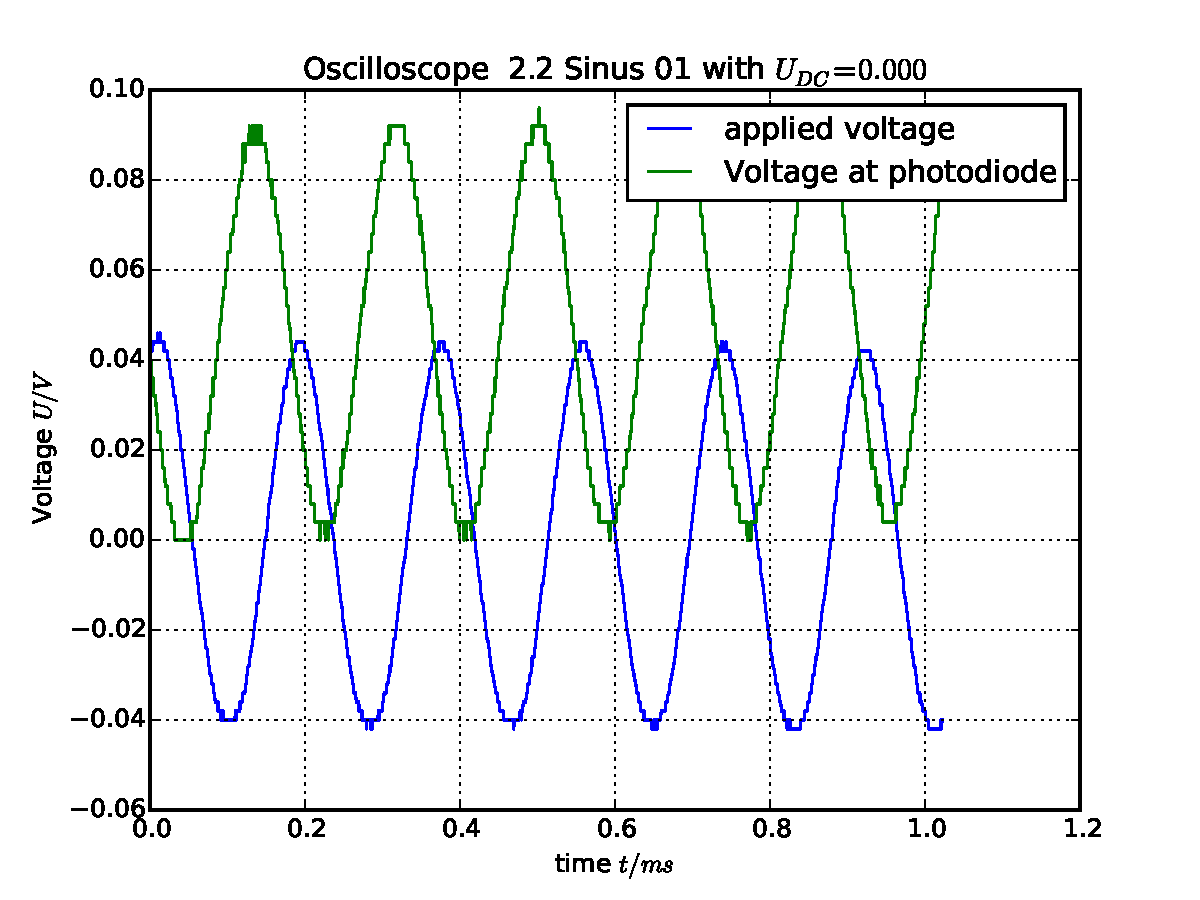
\includegraphics[width=15cm]{analysis/figures/22sinus01}
\end{figure}
\subsubsection{Sinus-generated Method: Applying Direct Current}
Now we will look at the inluence of different parameters on
the received signal, especially the effect of changing the
voltage. 
\paragraph{Important note:} After the measurements the
signalfrequency of the electrical field has gone up to 
$f=6.129$ khz! We noticed this without us to regulate this 
behavior. After the measurements we have changed this frequency in
order to the into account the change of frequency by adjusting.
We furthermore note that the change of frequency
does not seem to have a huge influence on the noisy regime except
that by reducing the frequency to $f=3.0$kHz we see the increase
of structure, meaning less noise and a clearly recognizable
sinusshape in the former noisy shape while the noisy regime
was shifted to other lower frequencies. We will look more refined
into this behavior in the next chapter.
\begin{figure}
    \begin{subfigure}[b]{\picwidth}
        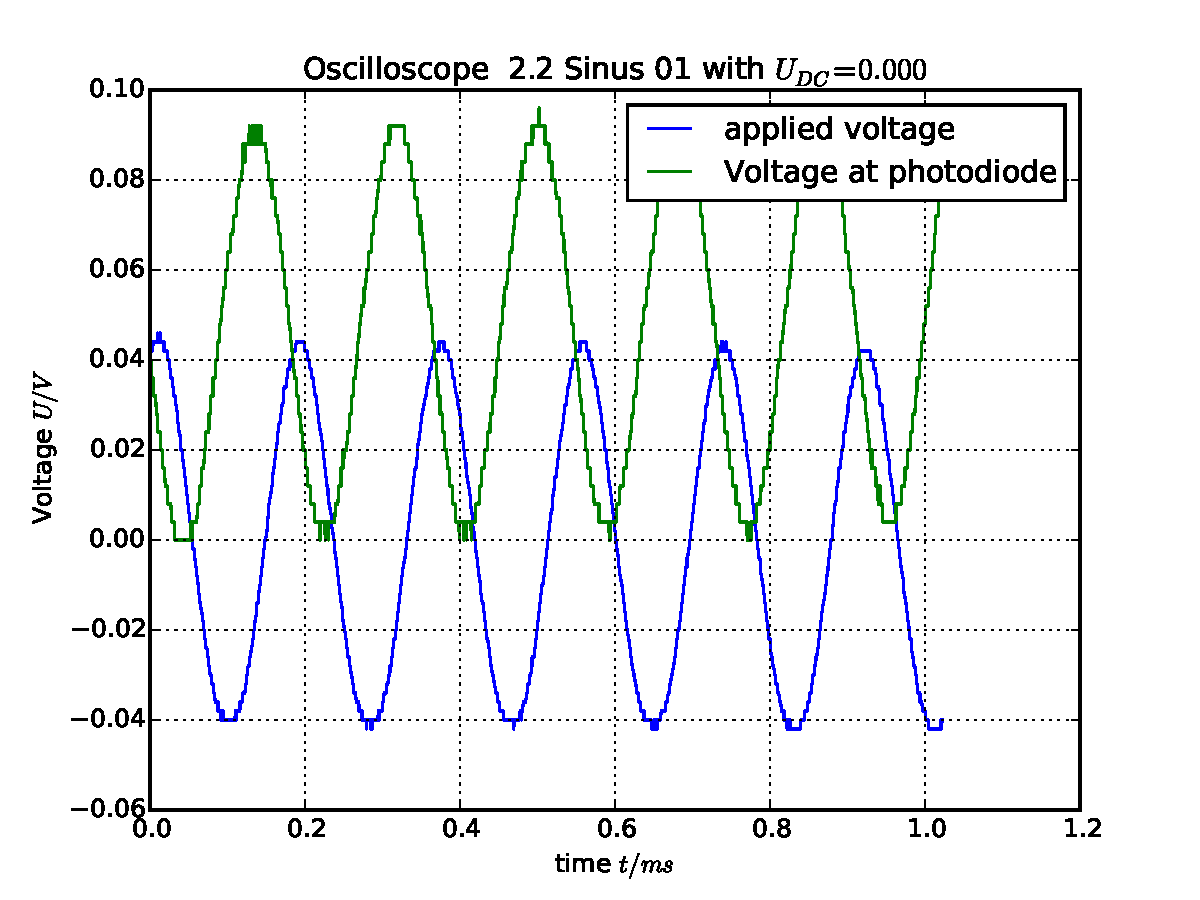
\includegraphics[width=\textwidth]{analysis/figures/22sinus01}
        \caption{}
    \end{subfigure}\qquad
    \begin{subfigure}[b]{\picwidth}
        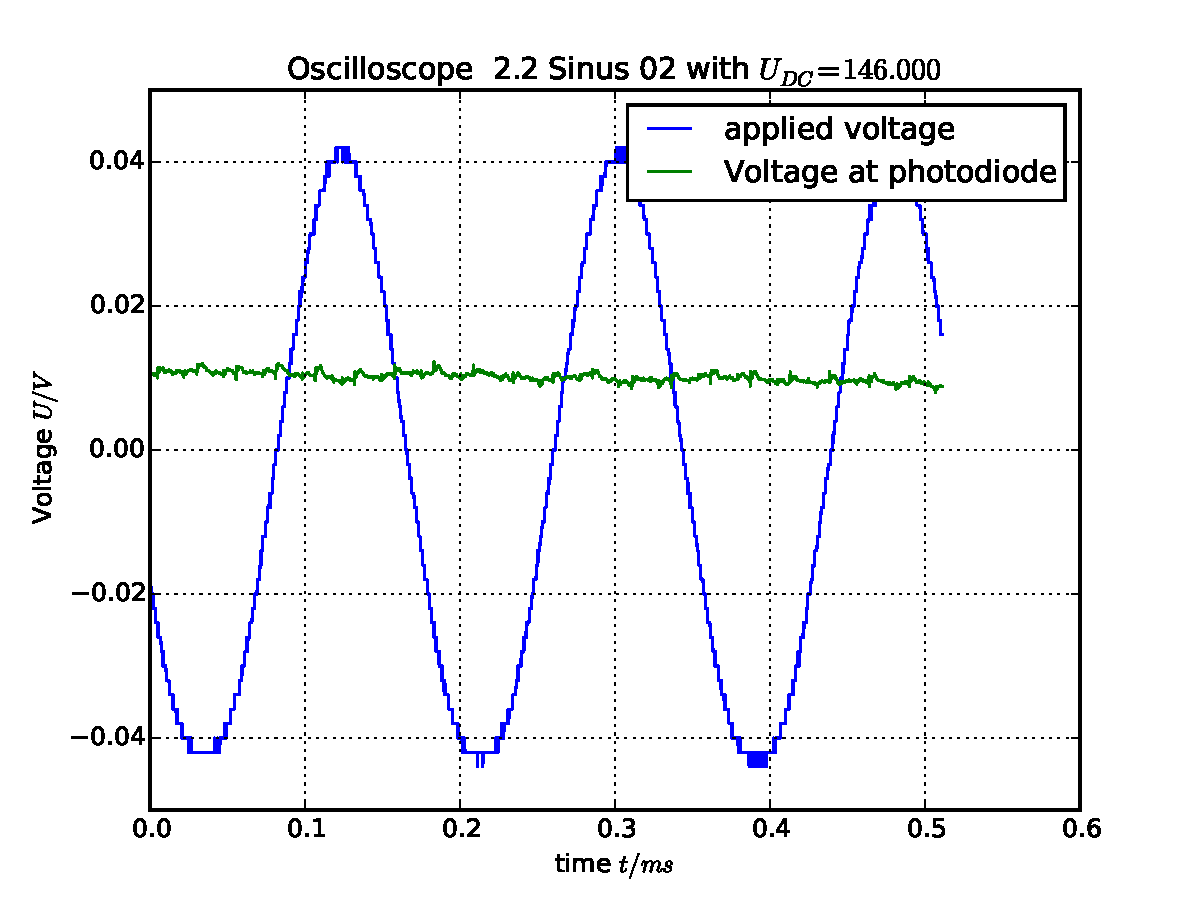
\includegraphics[width=\textwidth]{analysis/figures/22sinus02}
        \caption{}
    \end{subfigure}
    \begin{subfigure}[b]{\picwidth}
        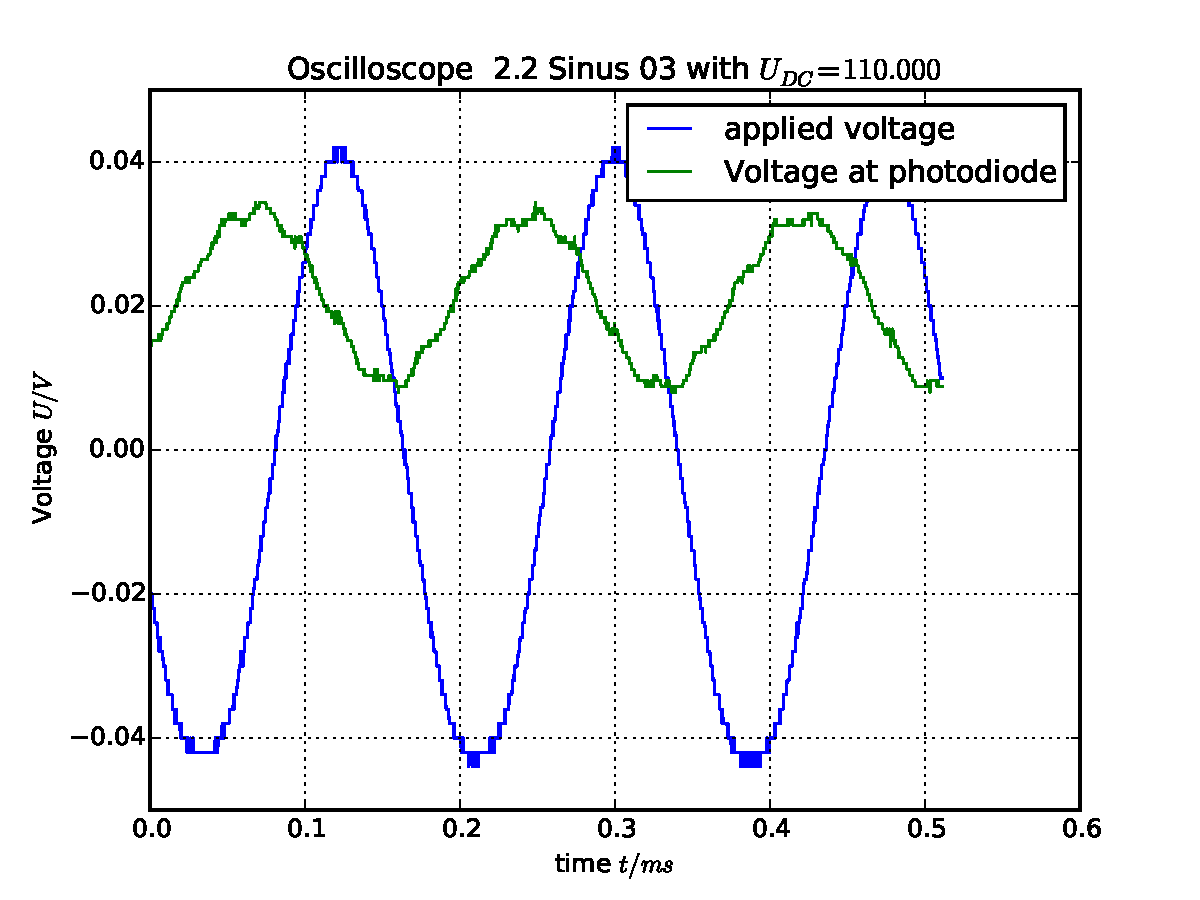
\includegraphics[width=\textwidth]{analysis/figures/22sinus03}
        \caption{}
    \end{subfigure}
    \begin{subfigure}[b]{\picwidth}
        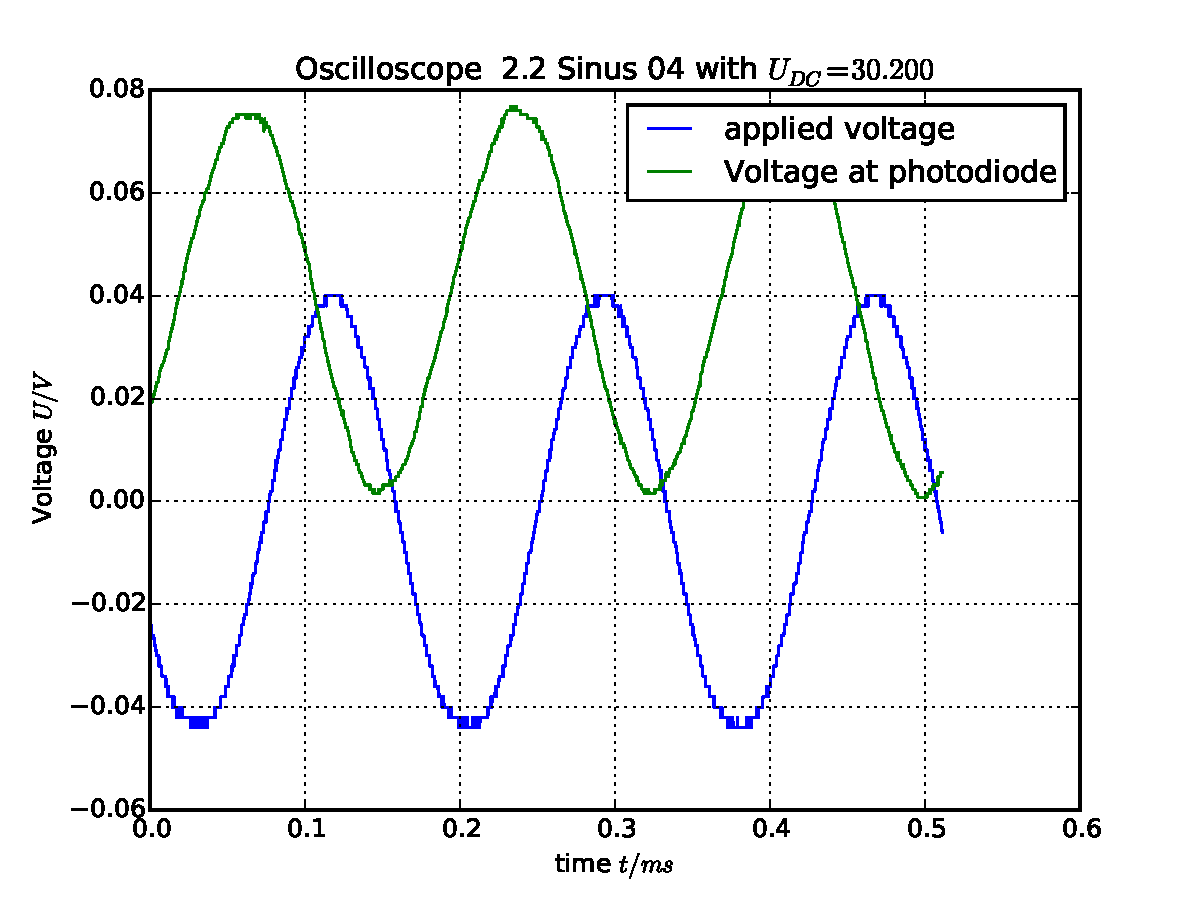
\includegraphics[width=\textwidth]{analysis/figures/22sinus04}
        \caption{}
    \end{subfigure}
    \begin{subfigure}[b]{\picwidth}
        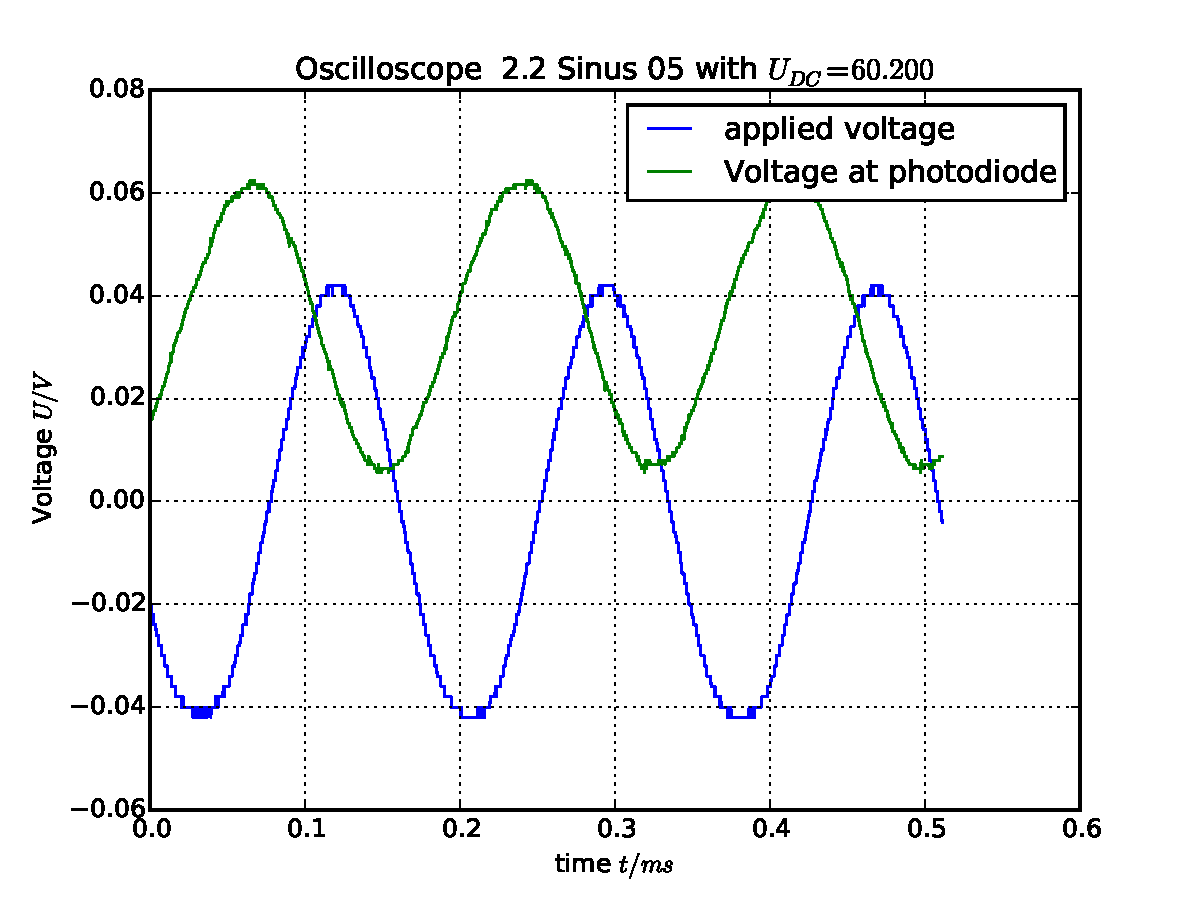
\includegraphics[width=\textwidth]{analysis/figures/22sinus05}
        \caption{}
    \end{subfigure}
    \begin{subfigure}[b]{\picwidth}
        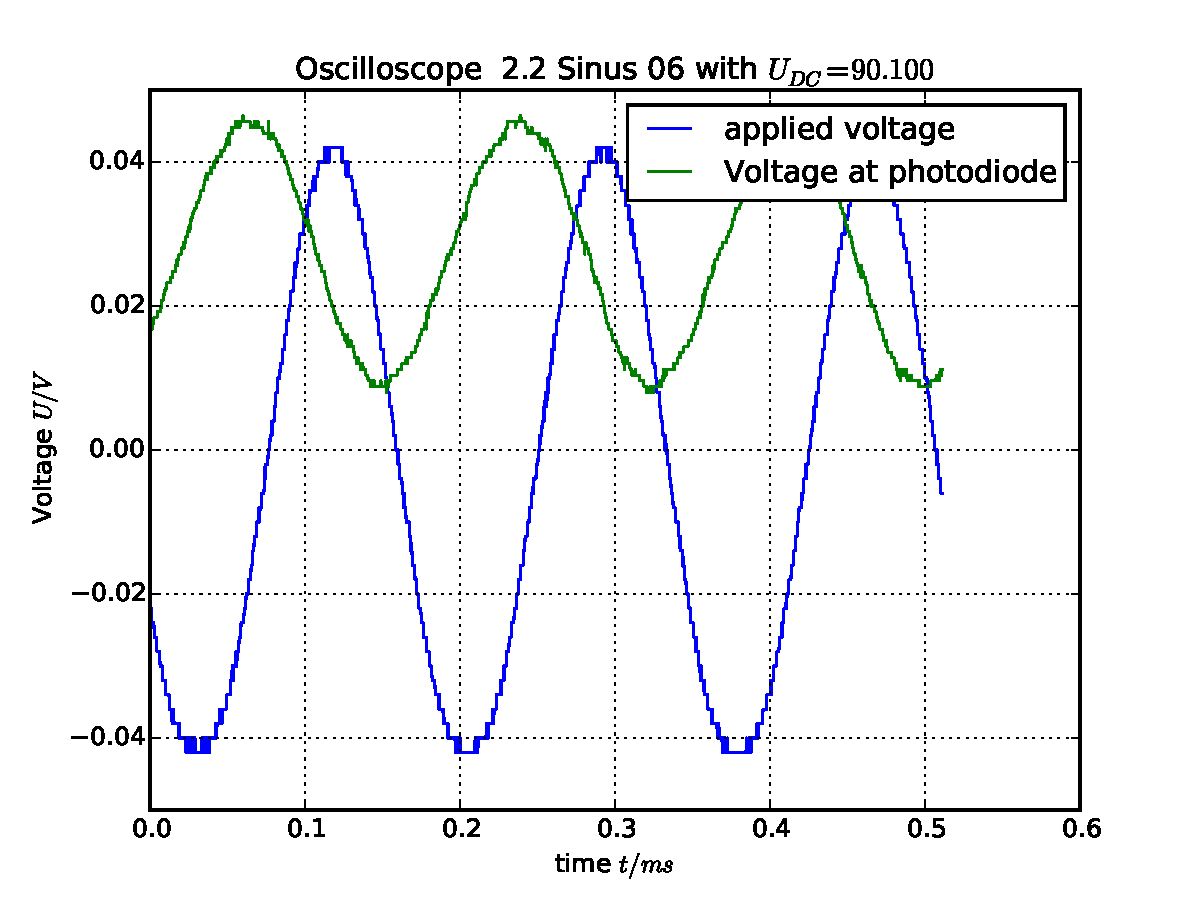
\includegraphics[width=\textwidth]{analysis/figures/22sinus06}
        \caption{}
    \end{subfigure}

    \caption{These series of figures show the impact of
        an applied sinussignal and a Direct Current with
        varying Voltage. In general we do not recognize huge 
        qualitative differences amongst those, but we will look
        later with a more refined analysis to it.}
    \label{fig:sinus1}
\end{figure}
\flushleft
\begin{figure}
    \begin{subfigure}[b]{\picwidth}
        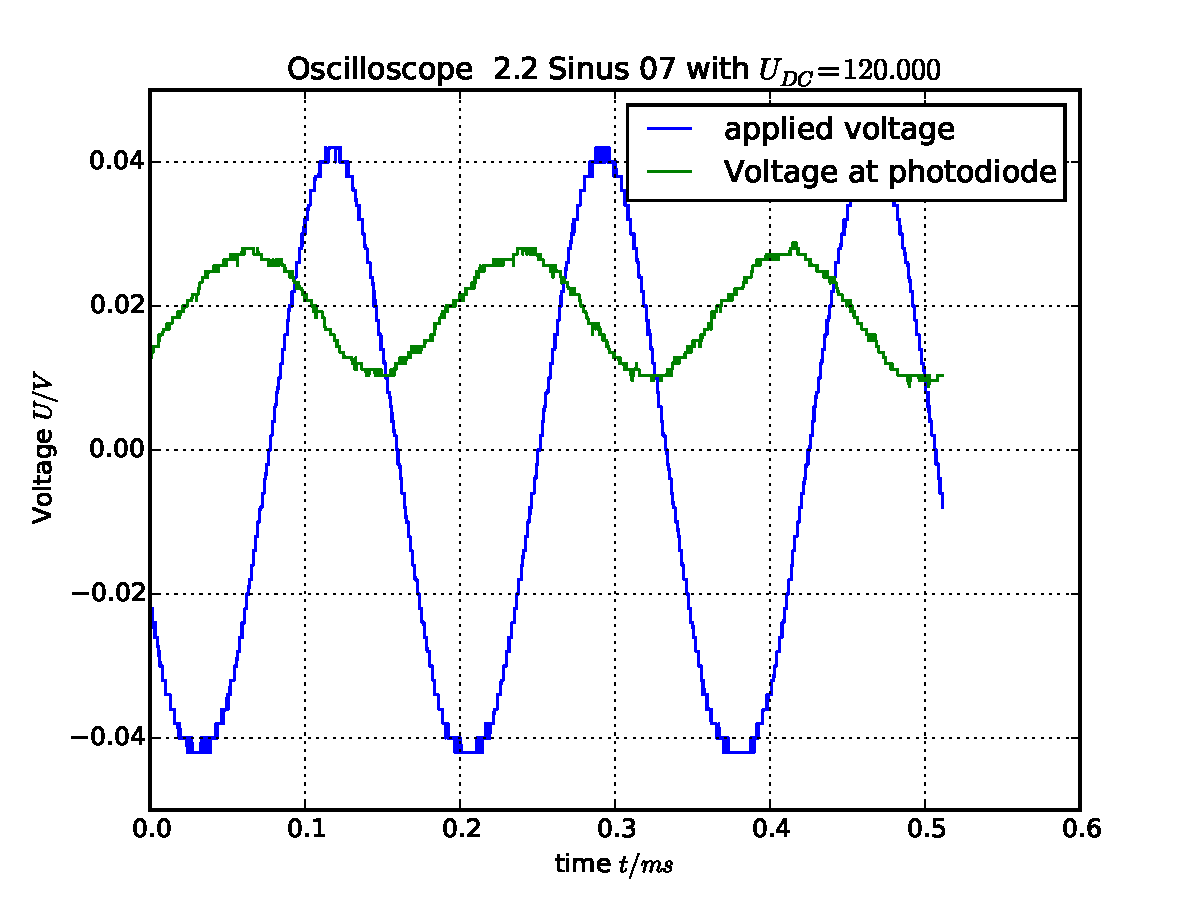
\includegraphics[width=\textwidth]{analysis/figures/22sinus07}
        \caption{}
    \end{subfigure}\qquad
    \begin{subfigure}[b]{\picwidth}
        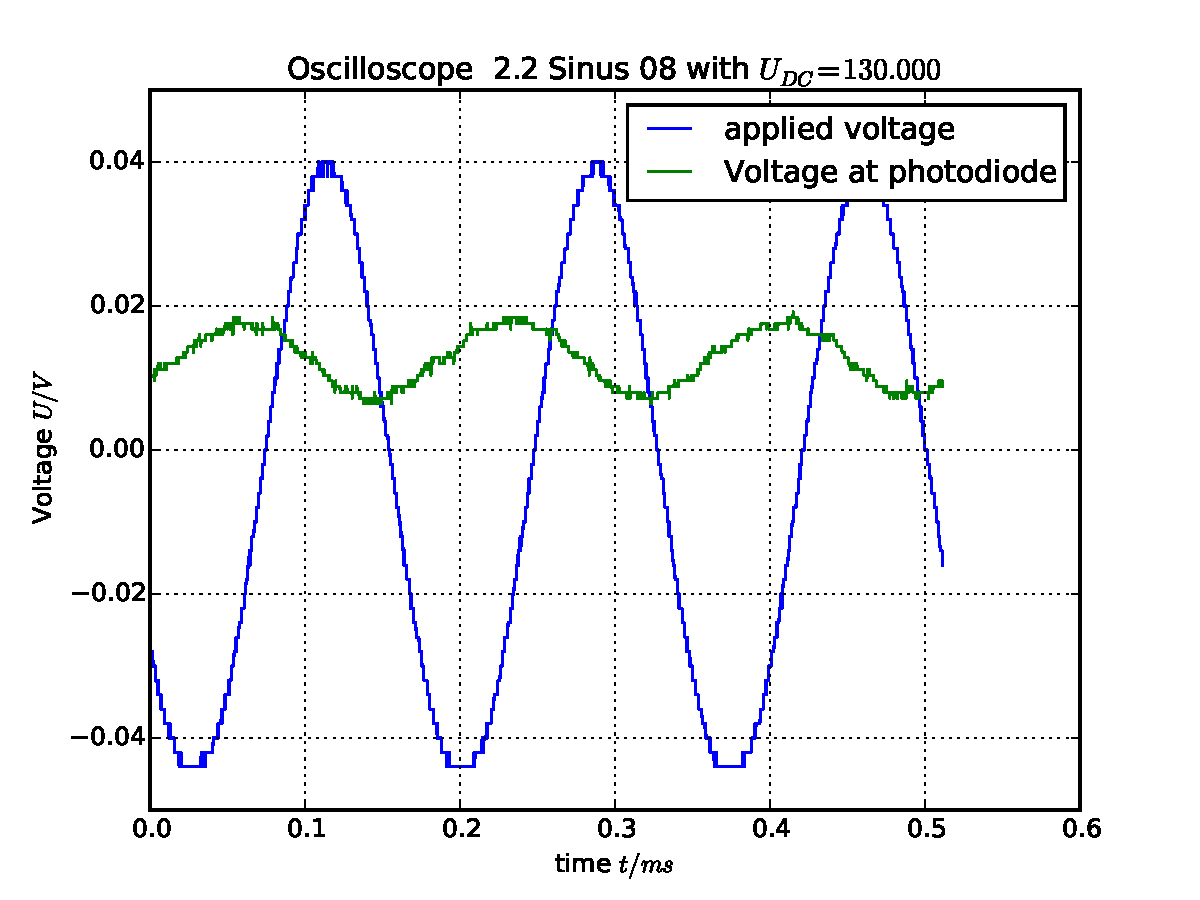
\includegraphics[width=\textwidth]{analysis/figures/22sinus08}
        \caption{}
    \end{subfigure}
    \begin{subfigure}[b]{\picwidth}
        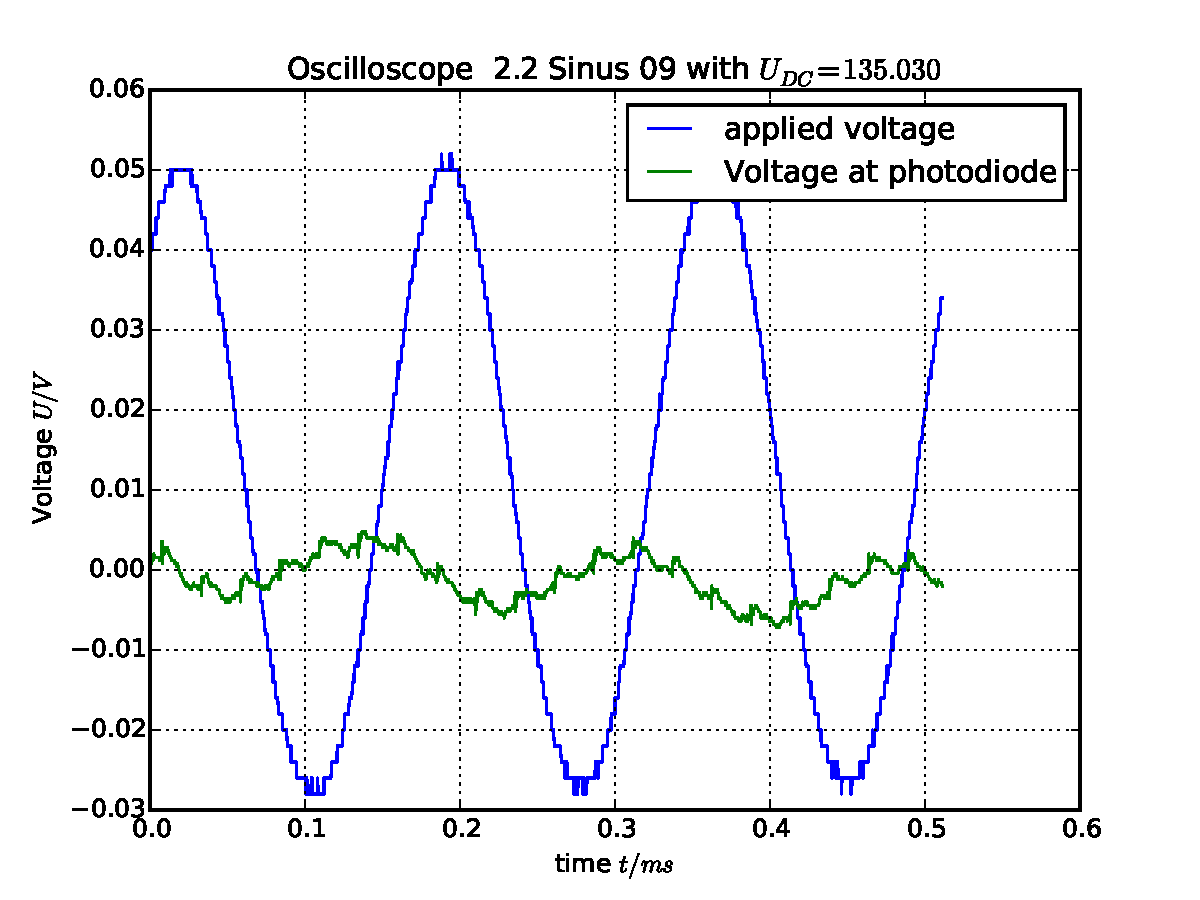
\includegraphics[width=\textwidth]{analysis/figures/22sinus09}
        \caption{}
    \end{subfigure}
    \begin{subfigure}[b]{\picwidth}
        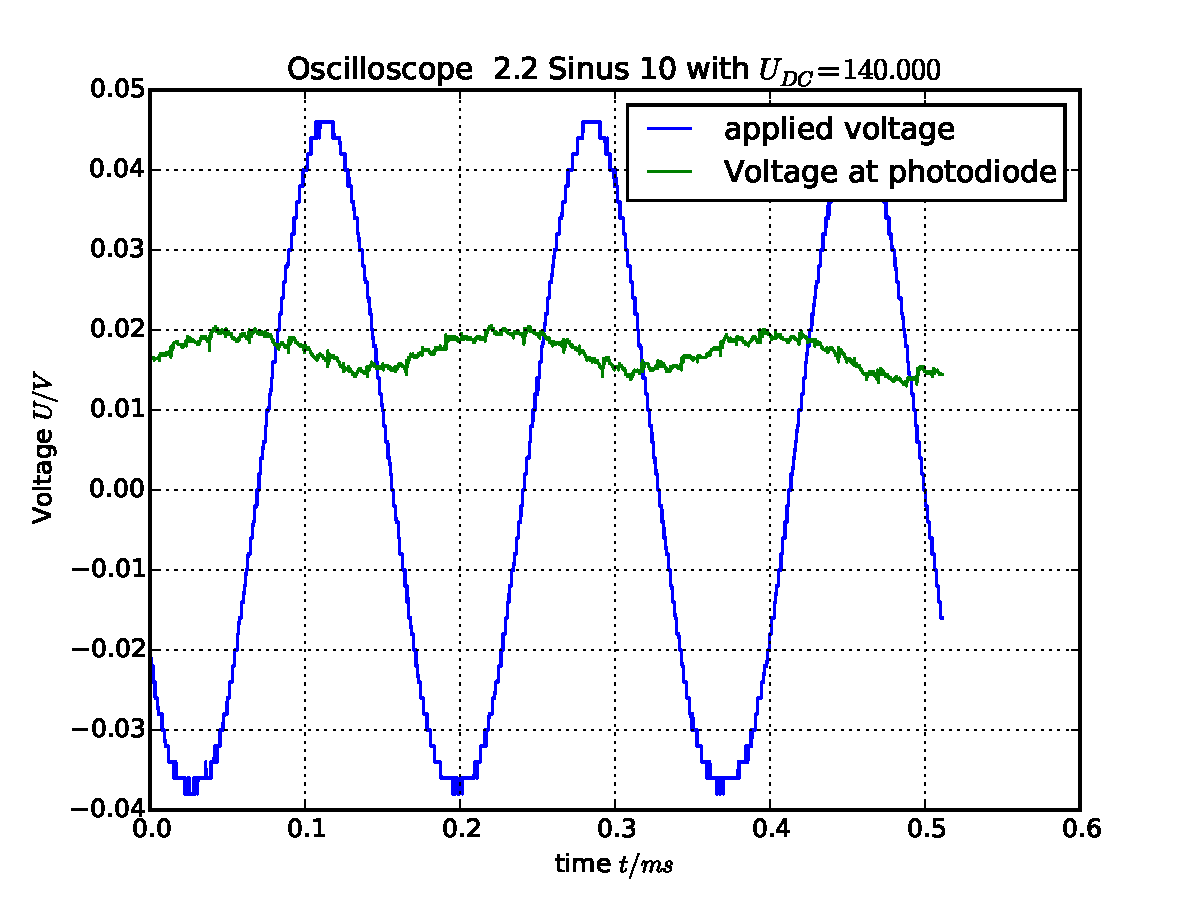
\includegraphics[width=\textwidth]{analysis/figures/22sinus10}
        \caption{}
    \end{subfigure}
    \begin{subfigure}[b]{\picwidth}
        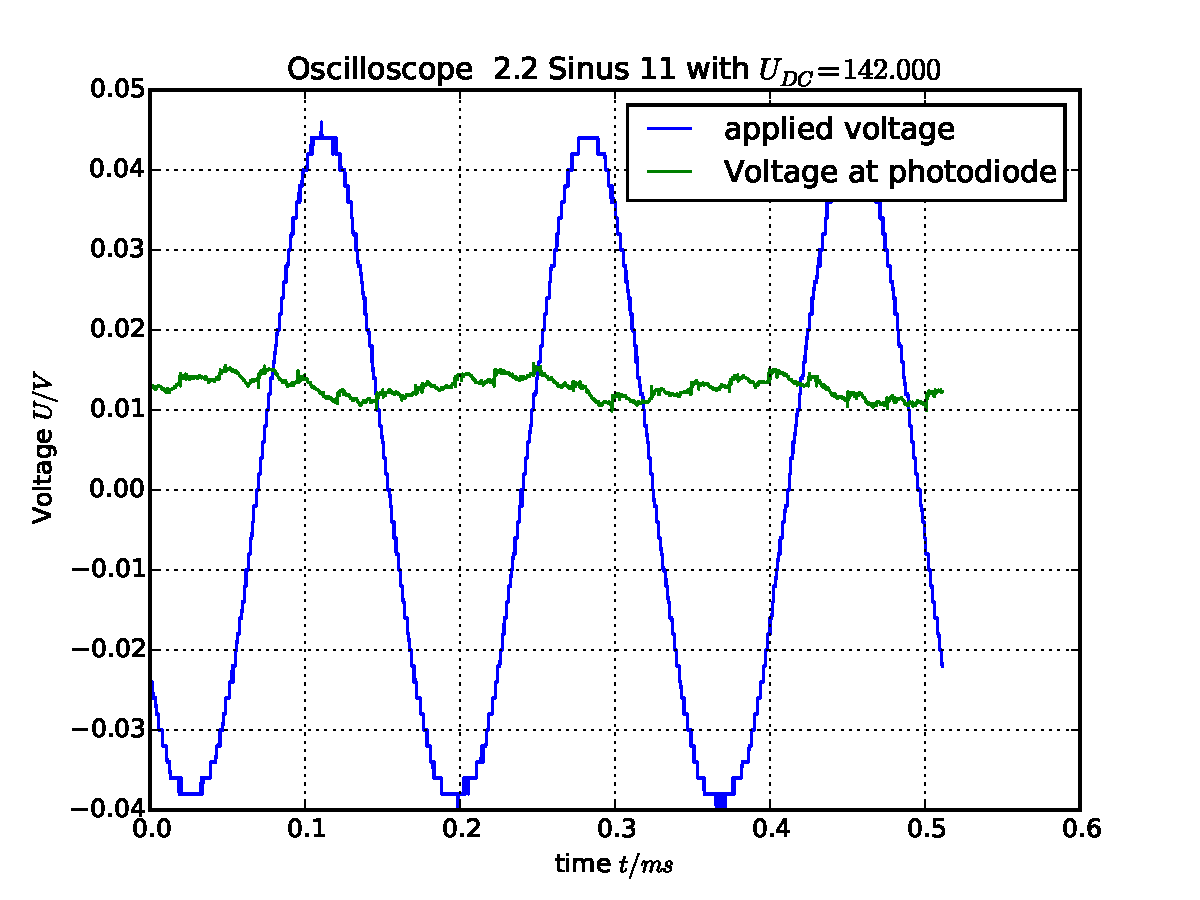
\includegraphics[width=\textwidth]{analysis/figures/22sinus11}
        \caption{}
    \end{subfigure}
    \begin{subfigure}[b]{\picwidth}
        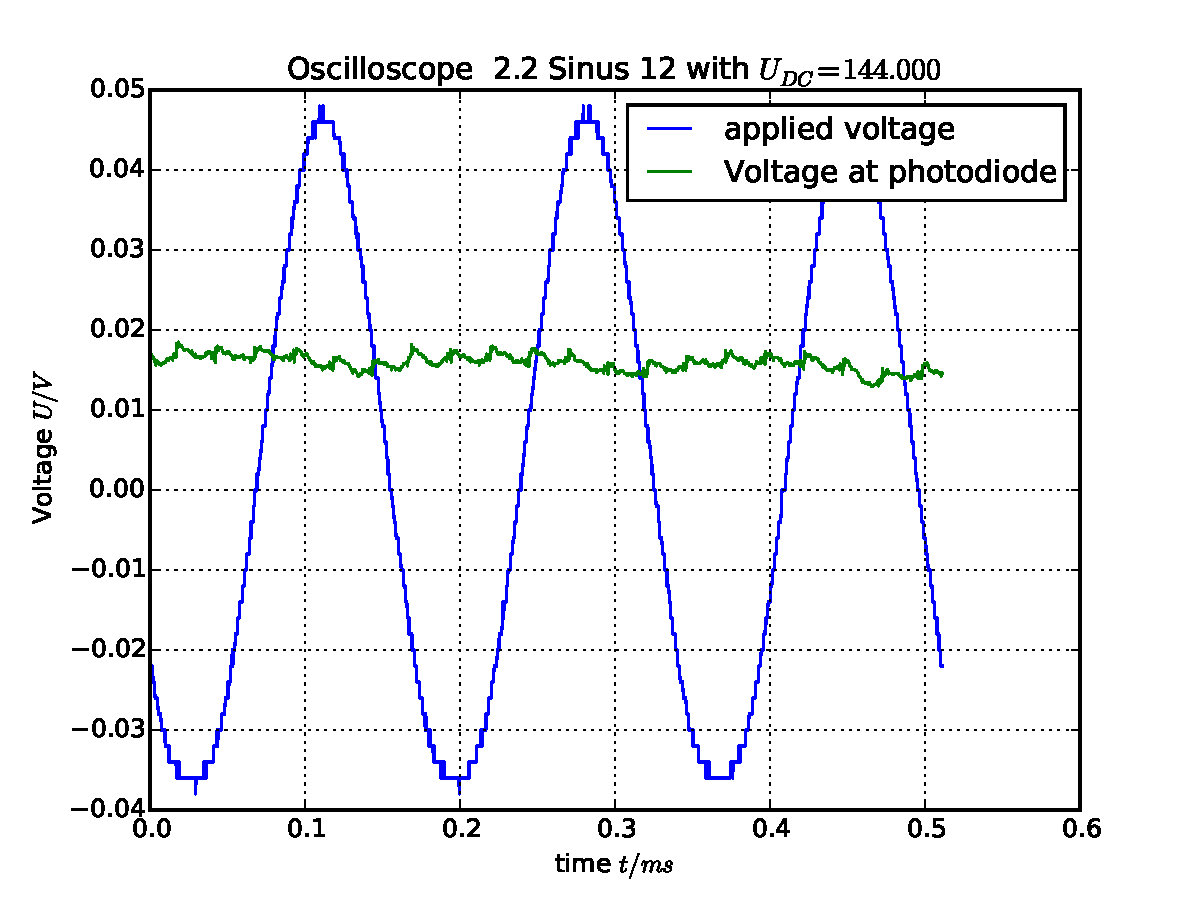
\includegraphics[width=\textwidth]{analysis/figures/22sinus12}
        \caption{}
    \end{subfigure}

    \caption{Now we enter the noisy regime in which we can 
        observe the effect of the state of the analysator. 
        Here we are indulged to find the noisiest curve in 
        order to check the range in which the $U_{\lambda / 2}$
        might be to find. As you will notice from the figures we
        suspect it to be in the range from $144.4V$ to $148.0V$
        but also see the next series of figures.}
    \label{fig:sinus2}
\end{figure}

\begin{figure}
    \begin{subfigure}[b]{\picwidth}
        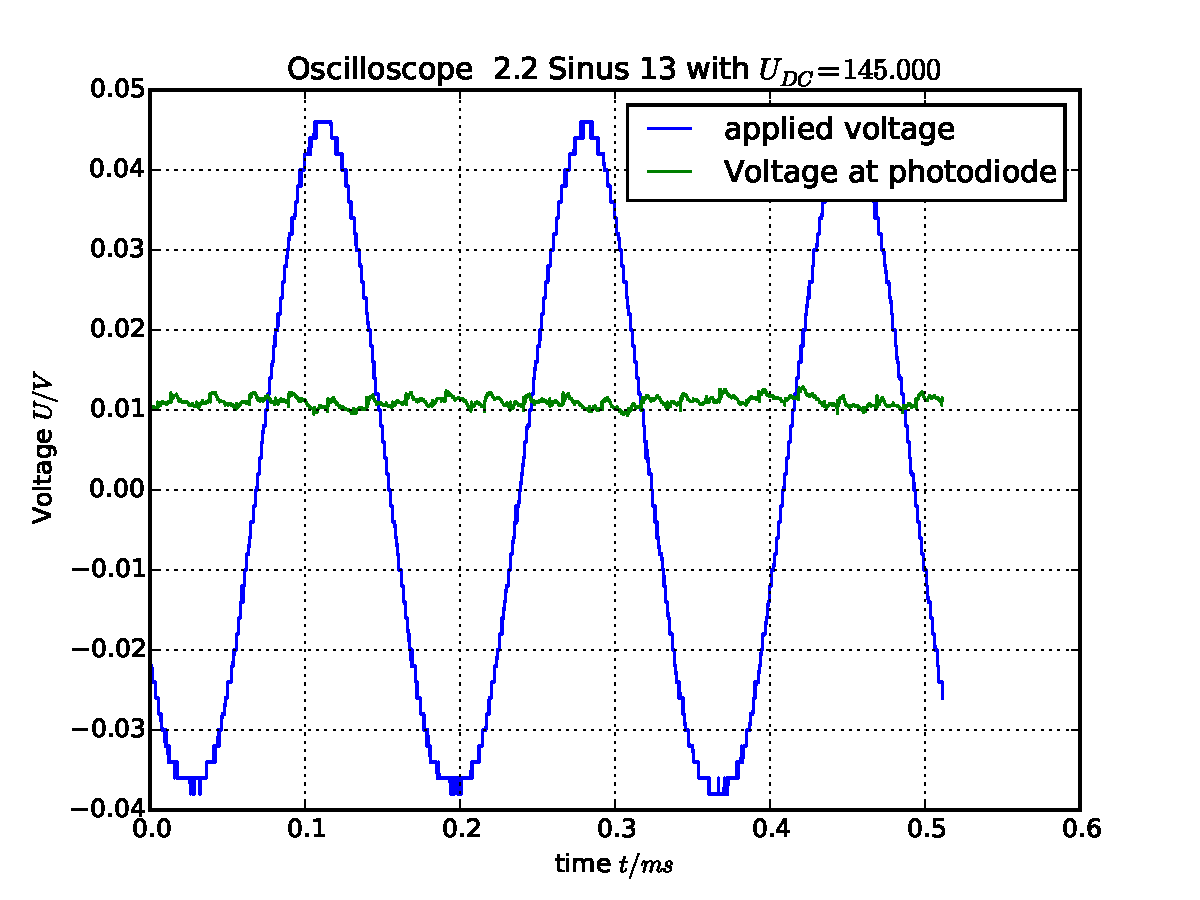
\includegraphics[width=\textwidth]{analysis/figures/22sinus13}
        \caption{}
    \end{subfigure}\qquad
    \begin{subfigure}[b]{\picwidth}
        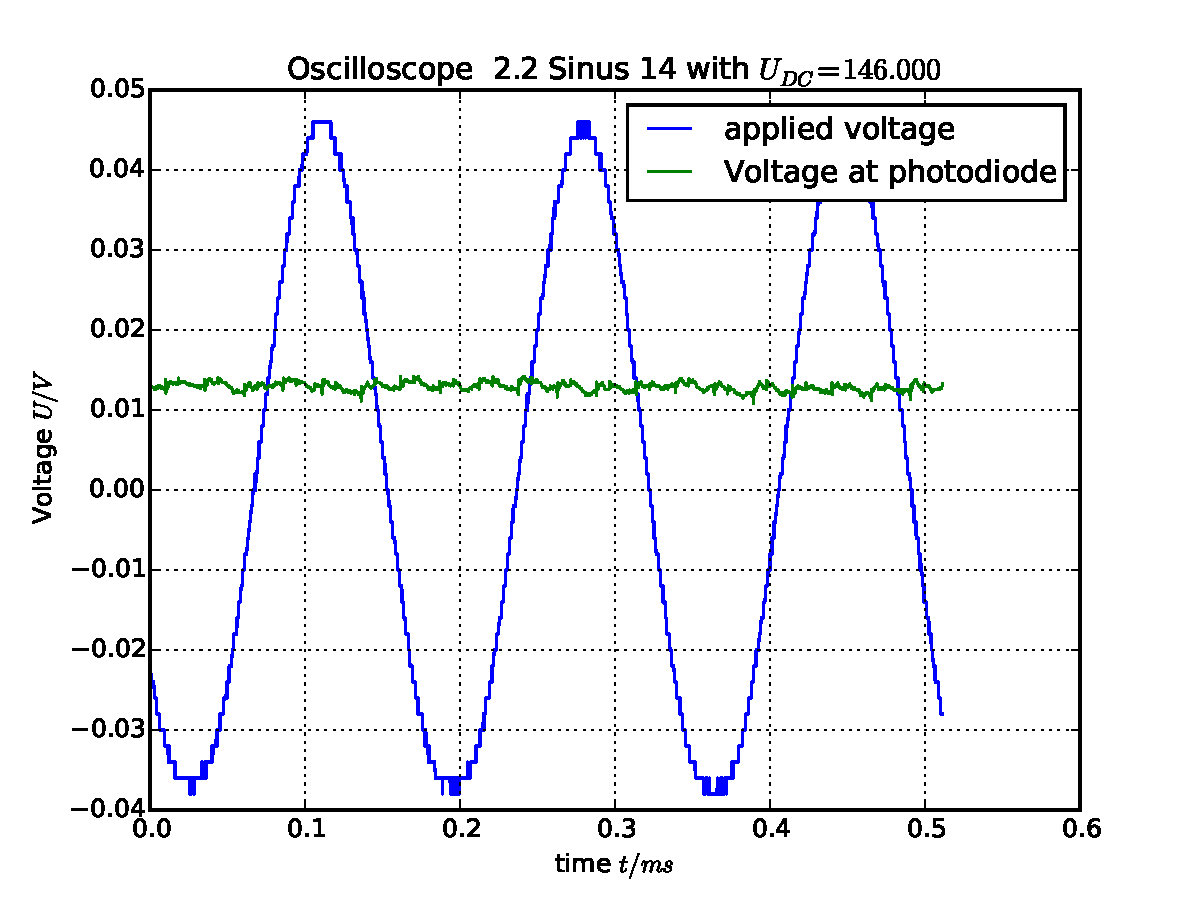
\includegraphics[width=\textwidth]{analysis/figures/22sinus14}
        \caption{}
    \end{subfigure}
    \begin{subfigure}[b]{\picwidth}
        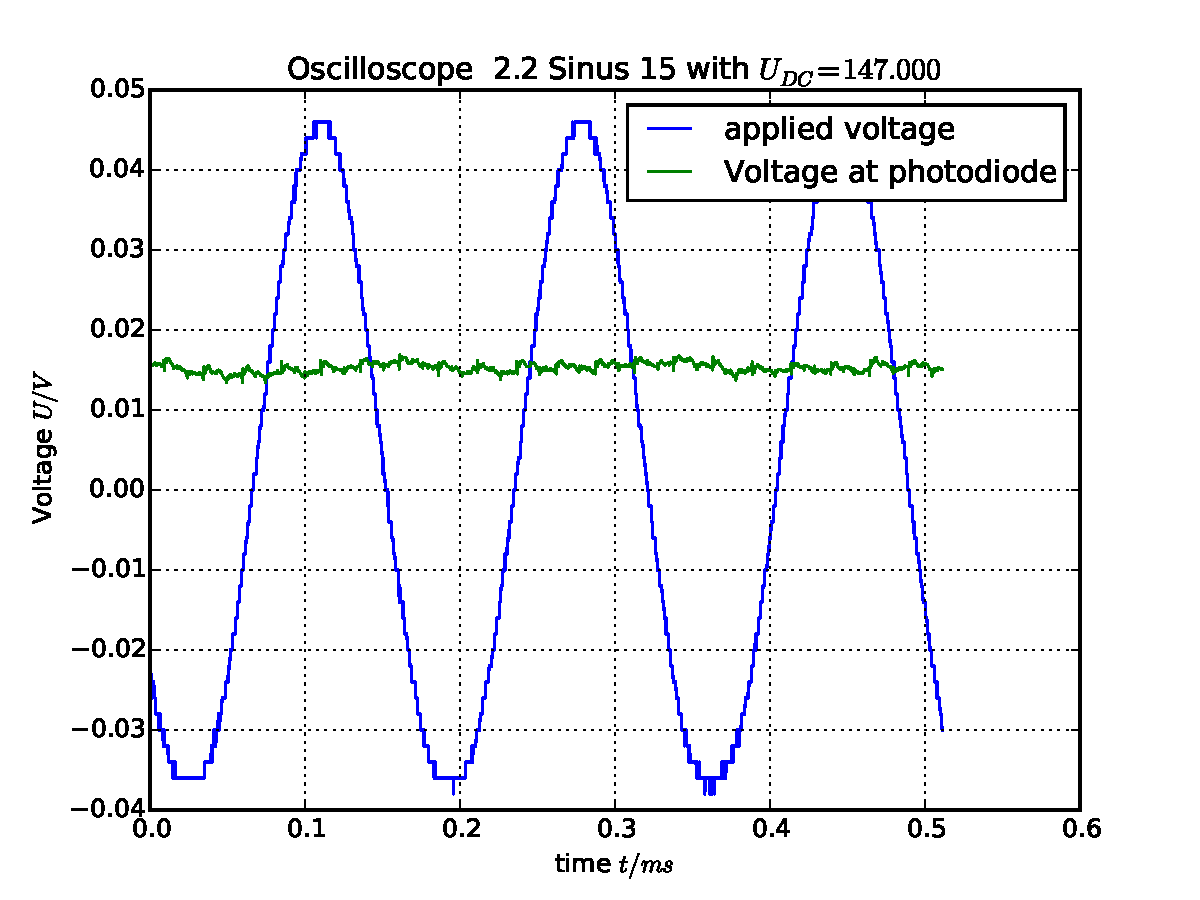
\includegraphics[width=\textwidth]{analysis/figures/22sinus15}
        \caption{}
    \end{subfigure}
    \begin{subfigure}[b]{\picwidth}
        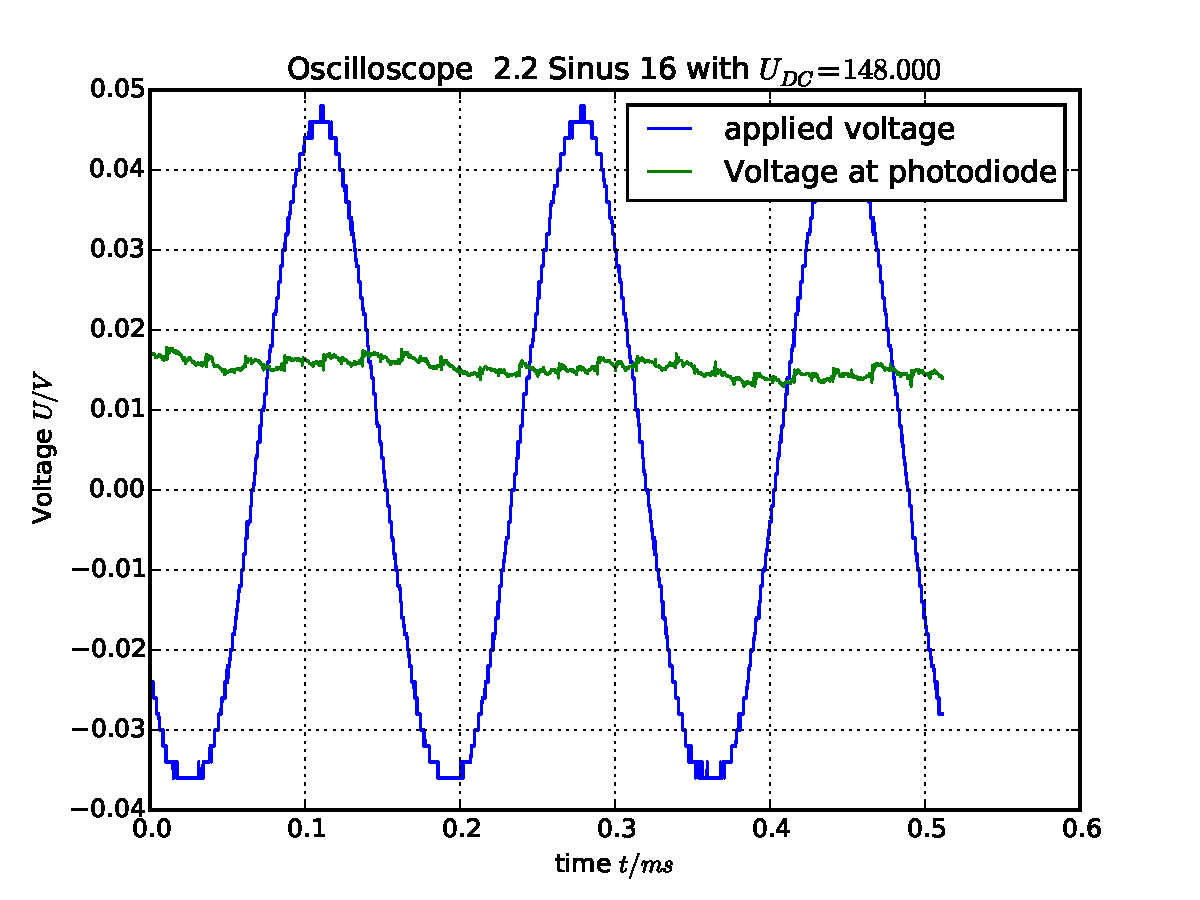
\includegraphics[width=\textwidth]{analysis/figures/22sinus16}
        \caption{}
    \end{subfigure}
    \begin{subfigure}[b]{\picwidth}
        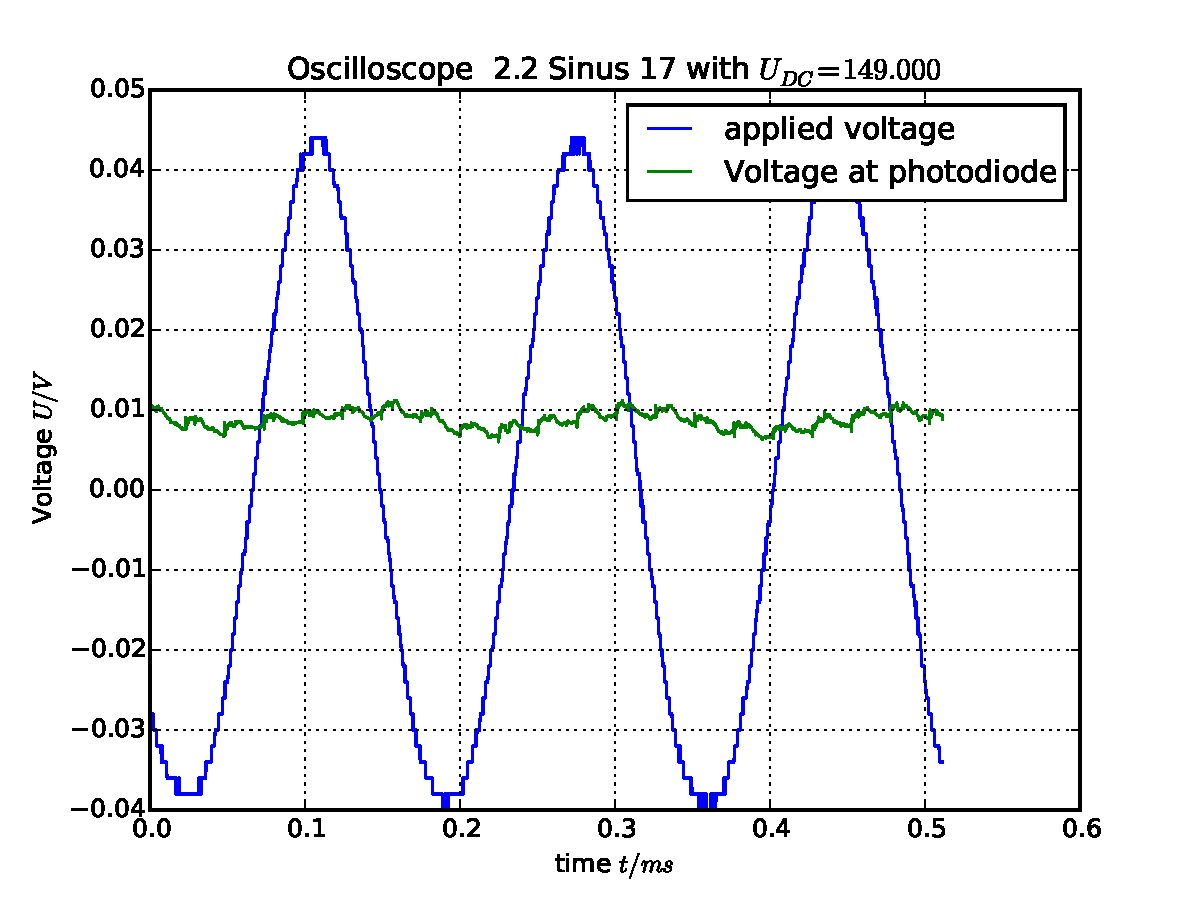
\includegraphics[width=\textwidth]{analysis/figures/22sinus17}
        \caption{}
    \end{subfigure}
    \begin{subfigure}[b]{\picwidth}
        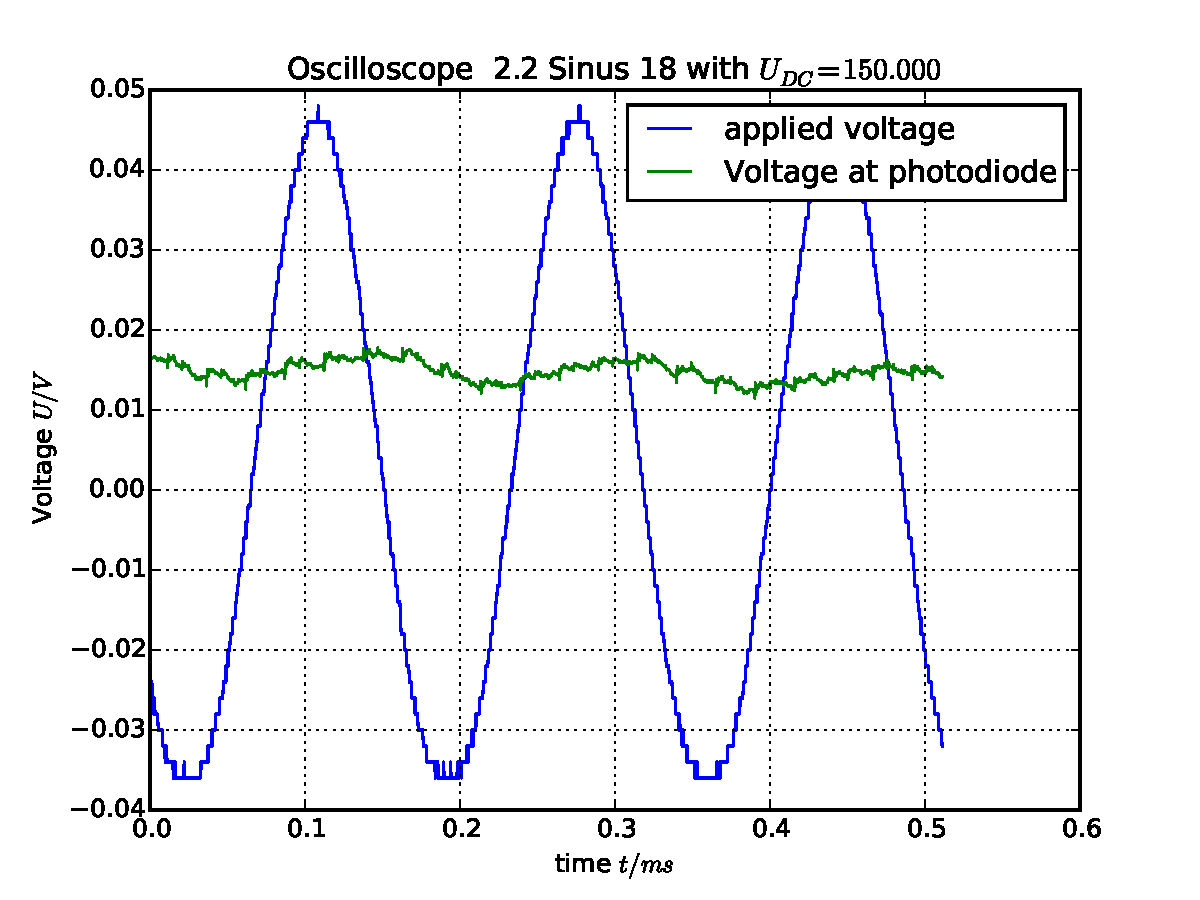
\includegraphics[width=\textwidth]{analysis/figures/22sinus18}
        \caption{}
    \end{subfigure}

    \caption{This is the noisy-regime, for explanation see
        Figure~\ref{fig:sinus2}. We have not seen any frequency
        doubling though.}
    \label{fig:sinus3}
\end{figure}

\begin{figure}
    \begin{subfigure}[b]{\picwidth}
        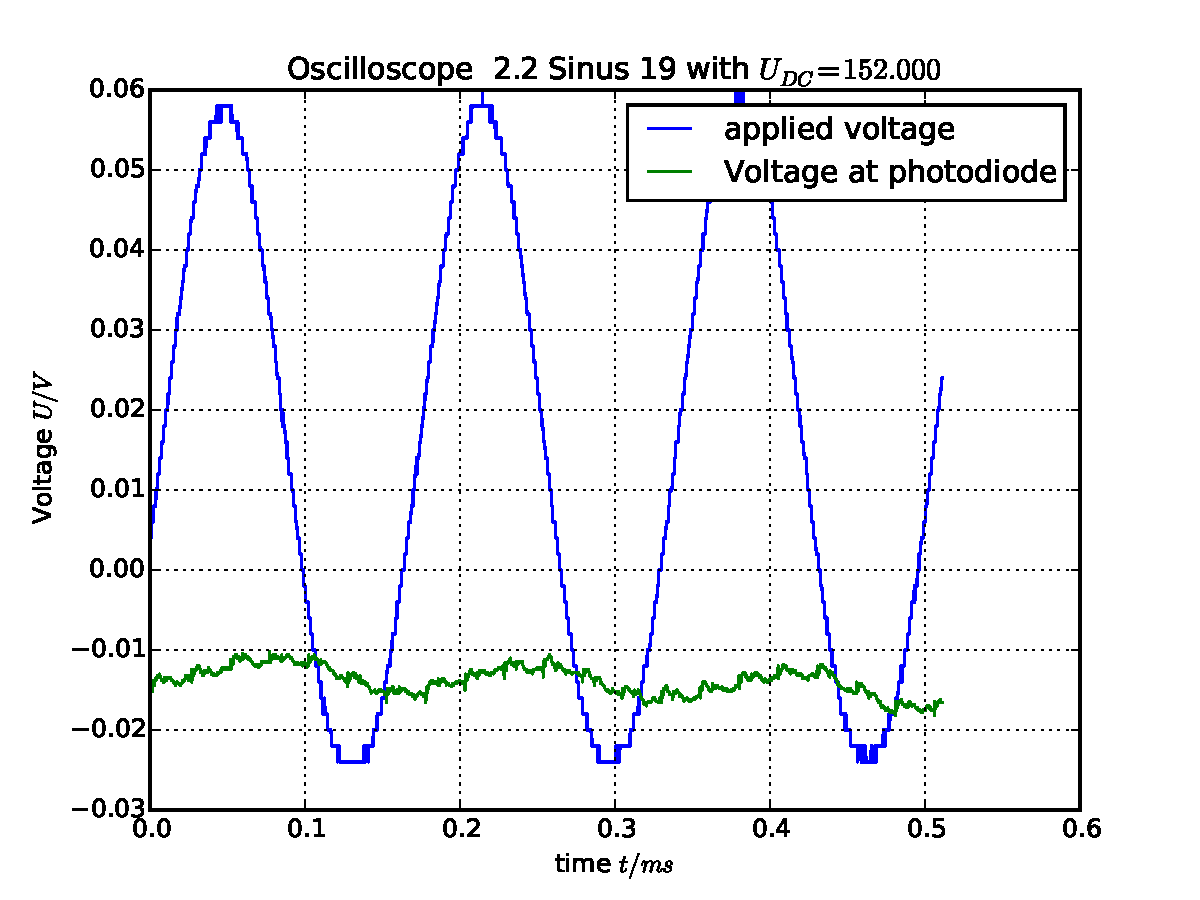
\includegraphics[width=\textwidth]{analysis/figures/22sinus19}
        \caption{}
    \end{subfigure}\qquad
    \begin{subfigure}[b]{\picwidth}
        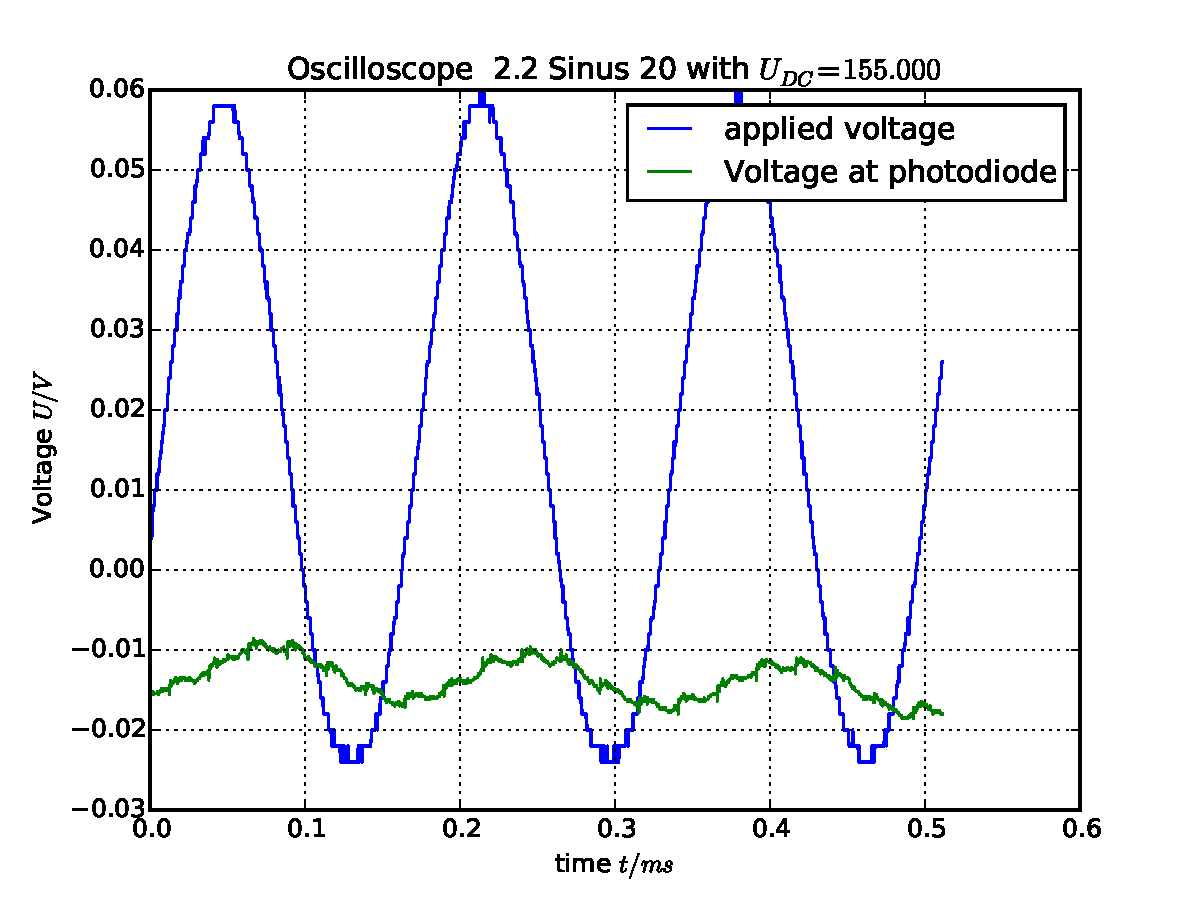
\includegraphics[width=\textwidth]{analysis/figures/22sinus20}
        \caption{}
    \end{subfigure}
    \begin{subfigure}[b]{\picwidth}
        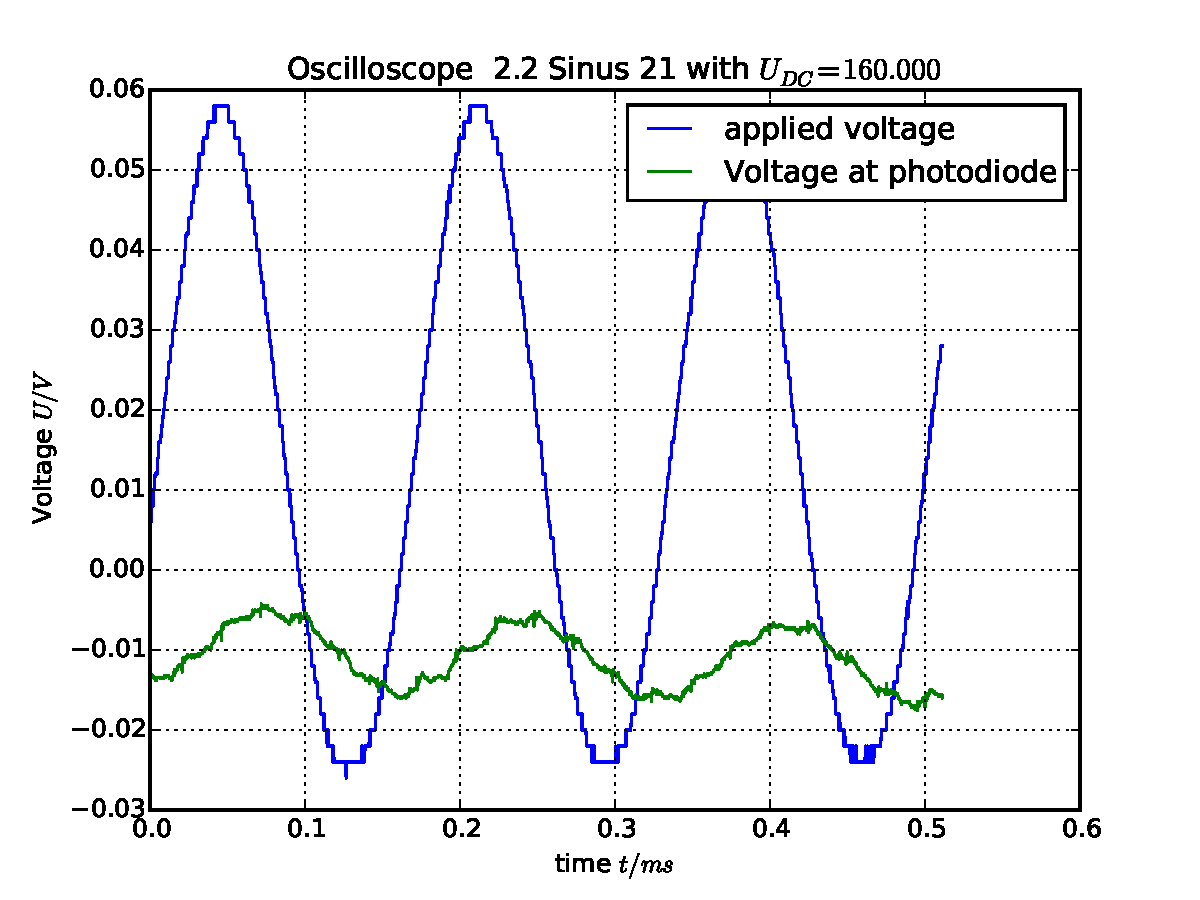
\includegraphics[width=\textwidth]{analysis/figures/22sinus21}
        \caption{}
    \end{subfigure}
    \begin{subfigure}[b]{\picwidth}
        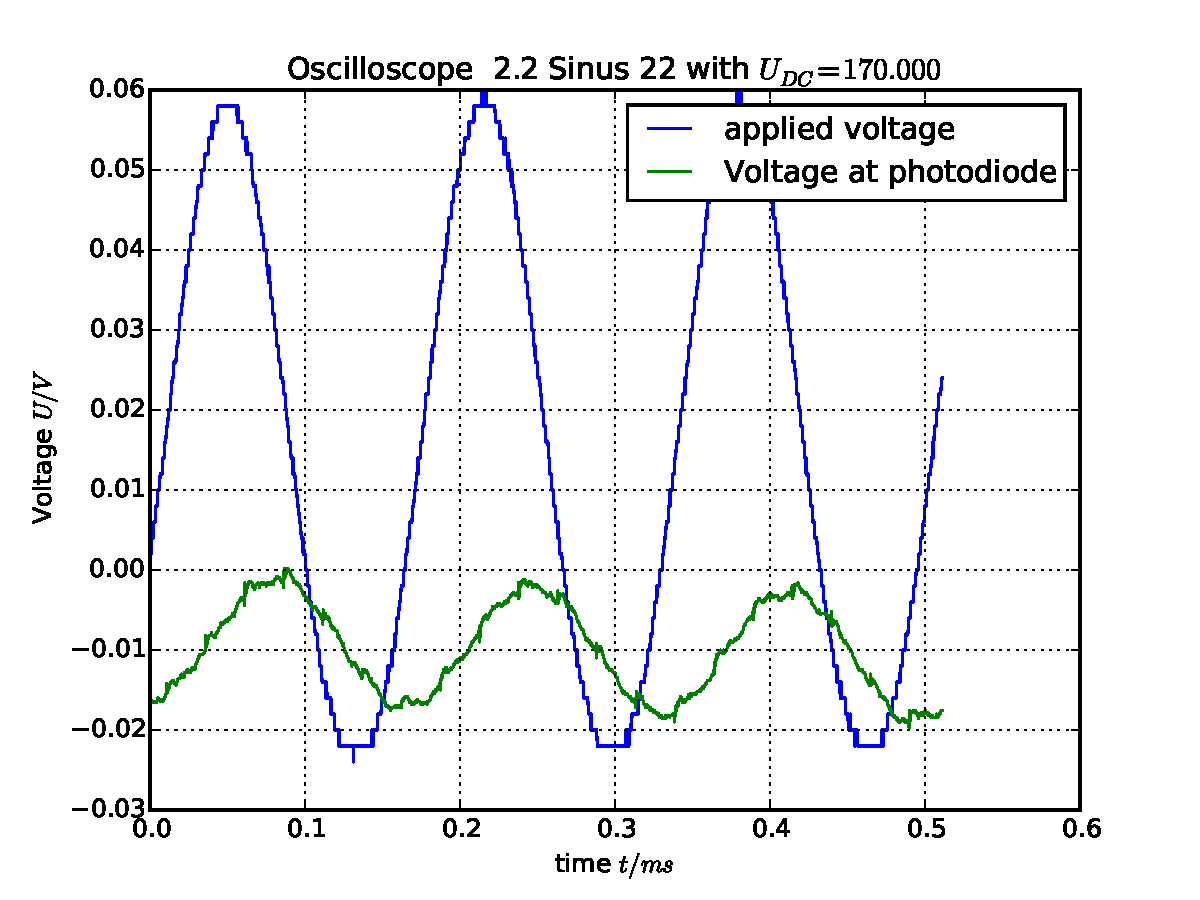
\includegraphics[width=\textwidth]{analysis/figures/22sinus22}
        \caption{}
    \end{subfigure}
    \begin{subfigure}[b]{\picwidth}
        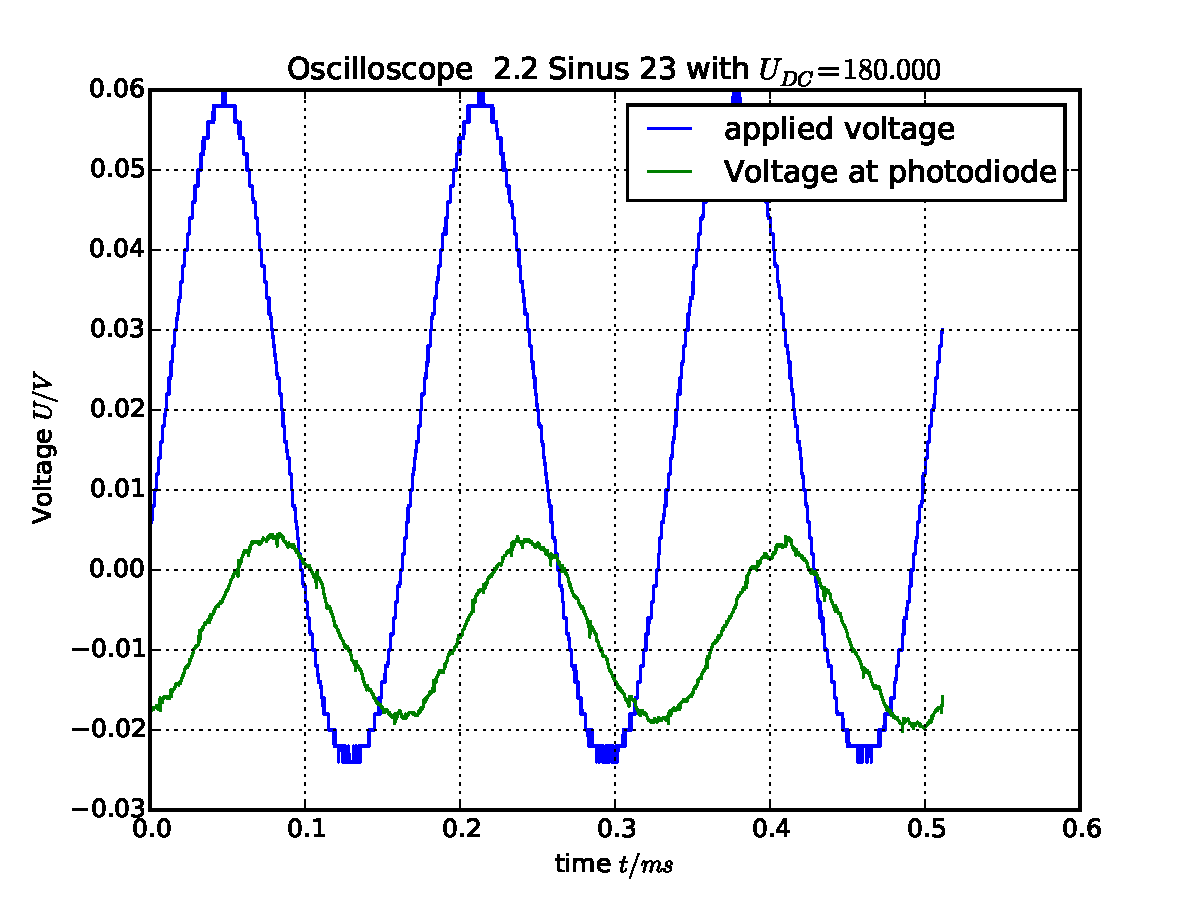
\includegraphics[width=\textwidth]{analysis/figures/22sinus23}
        \caption{}
    \end{subfigure}
    \begin{subfigure}[b]{\picwidth}
        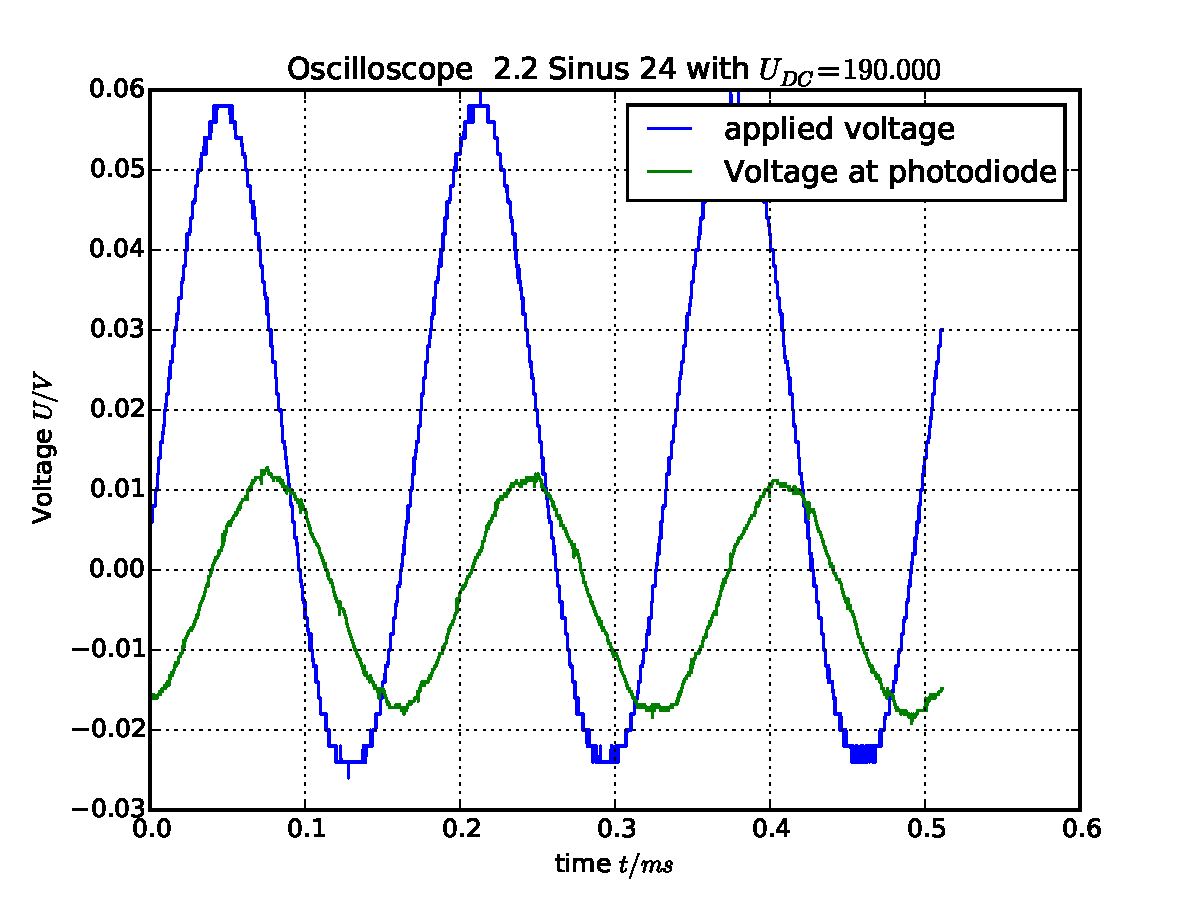
\includegraphics[width=\textwidth]{analysis/figures/22sinus24}
        \caption{}
    \end{subfigure}

    \caption{This series visualizes the upper limit and the end
        of the noisy regime, as more and more the sinusinput
        is dominating the shape of the signal with less noise.}
    \label{fig:sinus4}
\end{figure}
\clearpage
\subsubsection{Refined analysis of the impact of frequency on 
    the regime}
The figures in this section are accomplished with $U_{DC}=145.8 V$.
In this analysis we investigate the effect of the frequency
on the regime in which we get a rather noisy signal 

\begin{figure}
    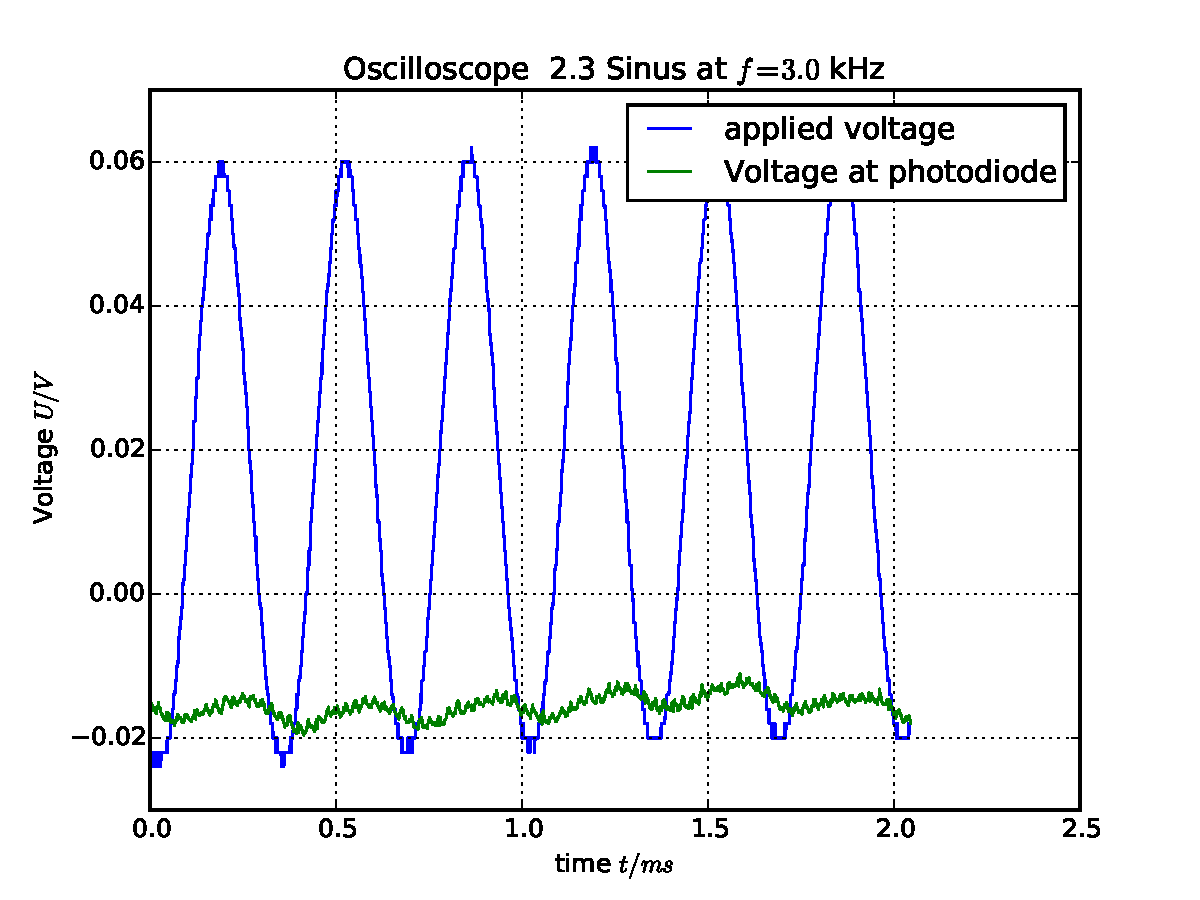
\includegraphics[width=15cm]{analysis/figures/23sinus01}
    \caption{In this figure we readjusted the frequency to
        $f=3.0$ kHz. In this figure we noticed, as already said
        in the last section, that the noisy regime was shifted
        to lower Voltage.}
\end{figure}

\begin{figure}
    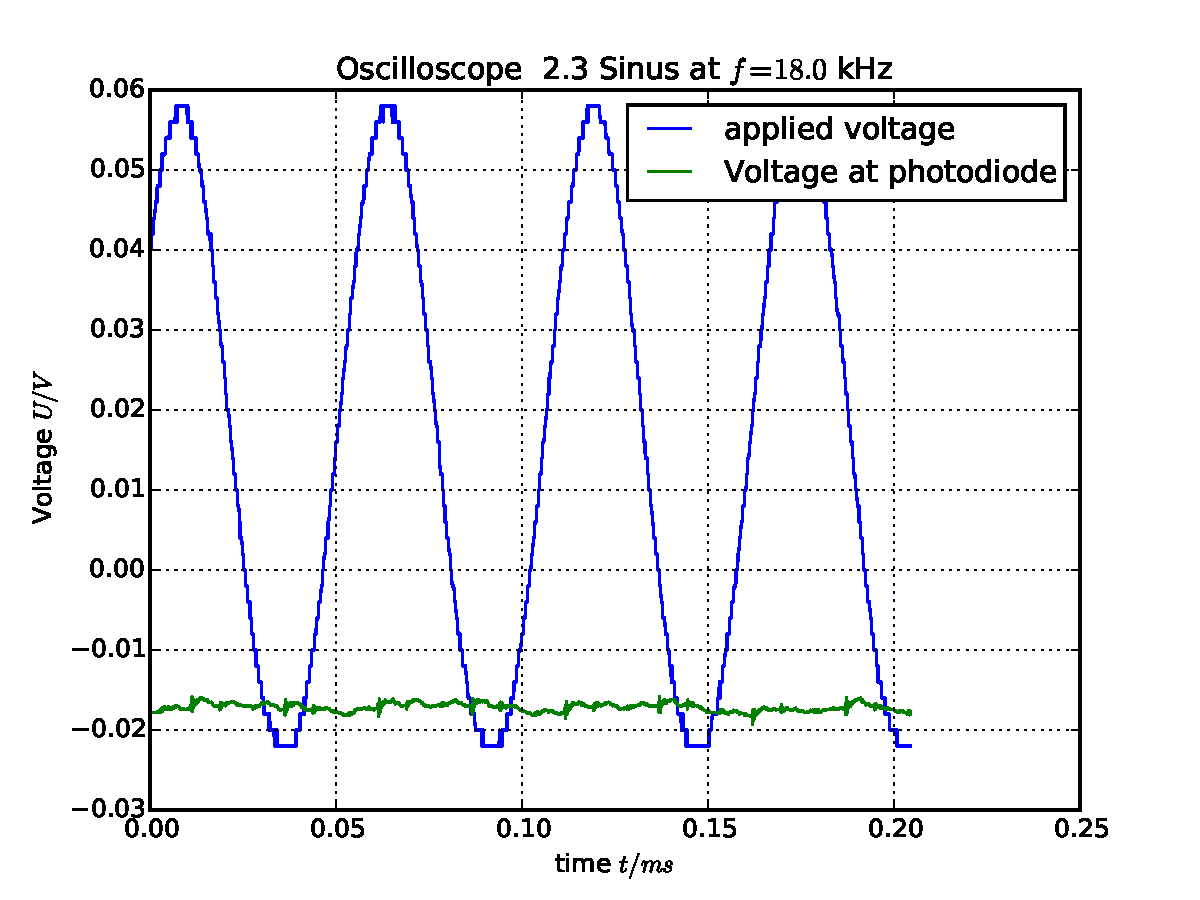
\includegraphics[width=15cm]{analysis/figures/23sinus02}
    \caption{At this level the regime of the voltage is shifted
        again, but in this case to a higher value. Unfortunatelly
        at this high frequency it is not possible to distinguish
        clearly between the different regimes because the signal
        is very noisy at all voltages (morelikely to shackle 
            or wiggle).}
\end{figure}

\begin{figure}
    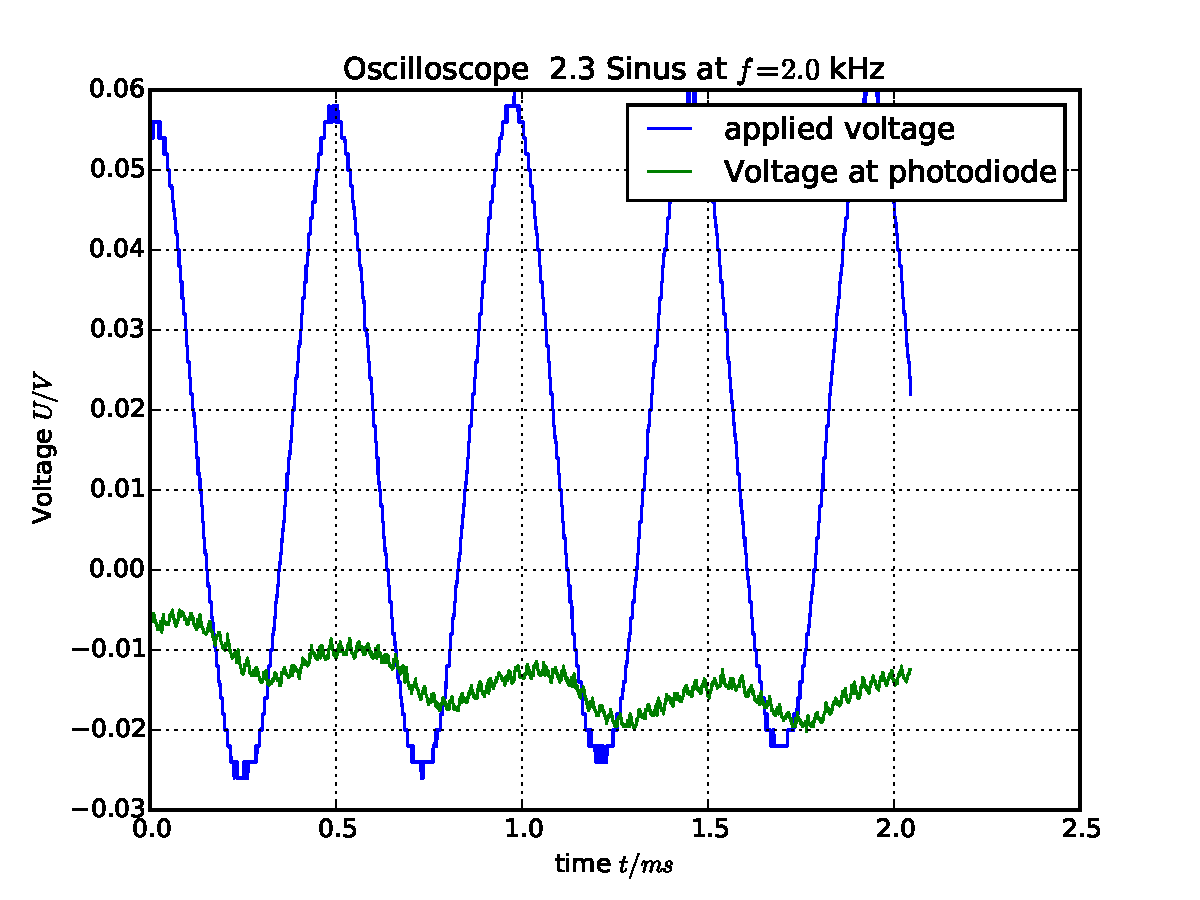
\includegraphics[width=15cm]{analysis/figures/23sinus03}
    \caption{}
\end{figure}

\clearpage
\subsubsection{Reanalysis with at the lower frequency}
